%% abtex2-modelo-trabalho-academico.tex, v-1.9.6 laurocesar
%% Copyright 2012-2016 by abnTeX2 group at http://www.abntex.net.br/ 
%%
%% This work may be distributed and/or modified under the
%% conditions of the LaTeX Project Public License, either version 1.3
%% of this license or (at your option) any later version.
%% The latest version of this license is in
%%   http://www.latex-project.org/lppl.txt
%% and version 1.3 or later is part of all distributions of LaTeX
%% version 2005/12/01 or later.
%%
%% This work has the LPPL maintenance status `maintained'.
%% 
%% The Current Maintainer of this work is the abnTeX2 team, led
%% by Lauro César Araujo. Further information are available on 
%% http://www.abntex.net.br/
%%
%% This work consists of the files abntex2-modelo-trabalho-academico.tex,
%% abntex2-modelo-include-comandos and abntex2-modelo-references.bib
%%

% ------------------------------------------------------------------------
% ------------------------------------------------------------------------
% abnTeX2: Modelo de Trabalho Academico (tese de doutorado, dissertacao de
% mestrado e trabalhos monograficos em geral) em conformidade com 
% ABNT NBR 14724:2011: Informacao e documentacao - Trabalhos academicos -
% Apresentacao
% ------------------------------------------------------------------------
% ------------------------------------------------------------------------

\documentclass[
	% -- opções da classe memoir --
	12pt,				% tamanho da fonte
	openany,			% capítulos começam em pág ímpar (insere página vazia caso preciso)
	twoside,			% para impressão em recto e verso. Oposto a oneside
	a4paper,			% tamanho do papel. 
	% -- opções da classe abntex2 --
	%chapter=TITLE,		% títulos de capítulos convertidos em letras maiúsculas
	%section=TITLE,		% títulos de seções convertidos em letras maiúsculas
	%subsection=TITLE,	% títulos de subseções convertidos em letras maiúsculas
	%subsubsection=TITLE,% títulos de subsubseções convertidos em letras maiúsculas
	% -- opções do pacote babel --
	english,			% idioma adicional para hifenização
	french,				% idioma adicional para hifenização
	spanish,			% idioma adicional para hifenização
	brazil				% o último idioma é o principal do documento
	]{abntex2}

% ---
% Pacotes básicos 
% ---
\usepackage{lmodern}			% Usa a fonte Latin Modern			
\usepackage[T1]{fontenc}		% Selecao de codigos de fonte.
\usepackage[utf8]{inputenc}		% Codificacao do documento (conversão automática dos acentos)
\usepackage{lastpage}			% Usado pela Ficha catalográfica
\usepackage{indentfirst}		% Indenta o primeiro parágrafo de cada seção.
\usepackage{color}				% Controle das cores
\usepackage{graphicx}			% Inclusão de gráficos
\usepackage{microtype} 			% para melhorias de justificação
% ---
\usepackage[utf8]{inputenc}
\usepackage{listings}
\usepackage{xcolor}
% Definindo novas cores
\definecolor{verde}{rgb}{0.25,0.5,0.35}
\definecolor{jpurple}{rgb}{0.5,0,0.35}
\definecolor{dkgreen}{rgb}{0,.6,0}
\definecolor{dkblue}{rgb}{0,0,.6}
\definecolor{dkyellow}{cmyk}{0,0,.8,.3}

% Configurando layout para mostrar codigos Java
\usepackage{listings}
\lstset{
     literate=%
         {á}{{\'a}}1
         {ã}{{\~a}}1
         {â}{{\^a}}1
         {í}{{\'i}}1
         {é}{{\'e}}1
         {ê}{{\^e}}1
         {ú}{{\'u}}1
         {ó}{{\'o}}1
         {õ}{{\~o}}1
}
\lstset{
  language=Java,
  basicstyle=\ttfamily\small,
  keywordstyle=\color{jpurple}\bfseries,
  stringstyle=\color{red},
  commentstyle=\color{verde},
  morecomment=[s][\color{blue}]{/**}{*/},
  extendedchars=true,
  showspaces=false,
  showstringspaces=false,
  numbers=left,
  numberstyle=\tiny,
  breaklines=true,
  backgroundcolor=\color{cyan!10},
  breakautoindent=true,
  captionpos=t,
  xleftmargin=0pt,
  tabsize=1
}
\lstdefinelanguage{XML}{
  basicstyle=\ttfamily\footnotesize,
  morestring=[b]",
  moredelim=[s][\bfseries\color{Maroon}]{<}{\ },
  moredelim=[s][\bfseries\color{Maroon}]{</}{>},
  moredelim=[l][\bfseries\color{Maroon}]{/>},
  moredelim=[l][\bfseries\color{Maroon}]{>},
  morecomment=[s]{<?}{?>},
  morecomment=[s]{<!--}{-->},
  commentstyle=\color{DarkOliveGreen},
  stringstyle=\color{blue},
  identifierstyle=\color{black}
}
% ---

		
% ---
% Pacotes adicionais, usados apenas no âmbito do Modelo Canônico do abnteX2
% ---
\usepackage{lipsum}				% para geração de dummy text
% ---

% ---
% Pacotes de citações
% ---
\usepackage[brazilian,hyperpageref]{backref}	 % Paginas com as citações na bibl
\usepackage[alf]{abntex2cite}	% Citações padrão ABNT
\usepackage{cite}
\usepackage{hyperref}
\usepackage{cleveref}
\setcounter{tocdepth}{5}

% --- 
% CONFIGURAÇÕES DE PACOTES
% --- 

% ---
% Configurações do pacote backref
% Usado sem a opção hyperpageref de backref
\renewcommand{\backrefpagesname}{Citado na(s) página(s):~}
% Texto padrão antes do número das páginas
\renewcommand{\backref}{}
% Define os textos da citação
\renewcommand*{\backrefalt}[4]{
	\ifcase #1 %
	%
	\or
		Citado na página #2.%
	\else
		Citado #1 vezes nas páginas #2.%
	\fi}%
% ---

% ---
% Informações de dados para CAPA e FOLHA DE ROSTO
% ---

\renewcommand{\imprimircapa}{
\thispagestyle{empty}

\vfill
 \begin{center}
    

    {\normalsize\bfseries \normalfont{UNIVERSIDADE FEDERAL FLUMINENSE}} \\
    {\normalsize\bfseries \normalfont{INSTITUTO DE CIÊNCIA E TECNOLOGIA}}\\
    {\normalsize\bfseries \normalfont{CURSO DE BACHARELADO EM CIÊNCIA DA COMPUTAÇÃO}}\\ 

    \vspace*{10cm}
    
    \large\bfseries{DESENVOLVIMENTO E USO DE UM APLICATIVO MÓVEL COMO ESTRATÉGIA DE EDUCAÇÃO AMBIENTAL}\\
    \vspace*{5cm}
    \noindent \\
    
    \begin{large} \bfseries \normalfont{Flávio Telles Paschoal Santos} \end{large}\\[0.4in]
    \vfill
    \normalsize\bfseries{ RIO DAS OSTRAS \\ 2021}
\end{center}

\normalsize



}

\renewcommand{\imprimirfolhaderosto}{

\begin{center}

 {\normalsize\bfseries \normalfont{UNIVERSIDADE FEDERAL FLUMINENSE}} \\
    {\normalsize\bfseries \normalfont{INSTITUTO DE CIÊNCIA E TECNOLOGIA}}\\
    {\normalsize\bfseries \normalfont{CURSO DE BACHARELADO EM CIÊNCIA DA COMPUTAÇÃO}}\\ 
    \vspace{3cm}
   \large\bfseries{DESENVOLVIMENTO E USO DE UM APLICATIVO MÓVEL COMO ESTRATÉGIA DE EDUCAÇÃO AMBIENTAL}\\
    \vspace{1cm}
    \hspace{.45\linewidth}
    \begin{minipage}{.50\linewidth}

            \textbf{\normalfont{Trabalho de conclusão de curso submetido ao Curso de Bacharelado em Ciência da Computação da Universidade Federal Fluminense, para a obtenção do Grau de Bacharel em Ciência da Computação.}}
    \end{minipage}
     \vspace{4cm}
     
      \begin{large} \bfseries {Flávio Telles Paschoal Santos}\end{large}\\[0.4in]
      \begin{large} \bfseries \normalfont{Orientador: Prof. Dr. Carlos Bazilio Martins}\end{large}\\[0.4in]
      \begin{large} \bfseries \normalfont{Coorientador: Prof. Dr. Flávio Machado}\end{large}\\[0.4in]
      
     


    \vspace{2cm}
    \vfill
    \normalsize\bfseries{ RIO DAS OSTRAS \\ 2021}
\end{center}

}
 
\titulo{Desenvolvimento e uso de um aplicativo móvel como estratégia de educação ambiental}
\autor{Flávio Telles Paschoal Santos}
\local{Rio das Ostras}
\data{2021}
\orientador{Carlos Bazilio}
\coorientador{Flávio Machado}
\tipotrabalho{Trabalho de conclusão de curso (Bacharelado)}
% O preambulo deve conter o tipo do trabalho, o objetivo, 
% o nome da instituição e a área de concentração 
\preambulo{Trabalho de conclusão de curso submetido ao Curso de Bacharelado em Ciência da Computação da Universidade Federal Fluminense, para a obtenção do Grau de Bacharel em Ciência da Computação.}
% ---


% ---
% Configurações de aparência do PDF final


% informações do PDF
\makeatletter
\hypersetup{
     	%pagebackref=true,
		pdftitle={\@title}, 
		pdfauthor={\@author},
    	pdfsubject={\imprimirpreambulo},
	    pdfcreator={LaTeX with abnTeX2},
		pdfkeywords={abnt}{latex}{abntex}{abntex2}{trabalho acadêmico}, 
		colorlinks=true,       		% false: boxed links; true: colored links
    	linkcolor=blue,          	% color of internal links
    	citecolor=blue,        		% color of links to bibliography
    	filecolor=magenta,      		% color of file links
		urlcolor=blue,
		bookmarksdepth=4
}
\makeatother
% --- 

% --- 
% Espaçamentos entre linhas e parágrafos 
% --- 

% O tamanho do parágrafo é dado por:
\setlength{\parindent}{1.3cm}

% Controle do espaçamento entre um parágrafo e outro:
\setlength{\parskip}{0.2cm}  % tente também \onelineskip

% ---
% compila o indice
% ---
\makeindex
% ---

% ----
% Início do documento
% ----
\begin{document}

% Seleciona o idioma do documento (conforme pacotes do babel)
%\selectlanguage{english}
\selectlanguage{brazil}

% Retira espaço extra obsoleto entre as frases.
\frenchspacing 

% ----------------------------------------------------------
% ELEMENTOS PRÉ-TEXTUAIS
% ----------------------------------------------------------
% \pretextual

% ---
% Capa
% ---
\imprimircapa
% ---

% ---
% Folha de rosto
% (o * indica que haverá a ficha bibliográfica)
% ---
\imprimirfolhaderosto

% ---



% ---
% Inserir folha de aprovação
% ---

% Isto é um exemplo de Folha de aprovação, elemento obrigatório da NBR
% 14724/2011 (seção 4.2.1.3). Você pode utilizar este modelo até a aprovação
% do trabalho. Após isso, substitua todo o conteúdo deste arquivo por uma
% imagem da página assinada pela banca com o comando abaixo:
%
% \includepdf{folhadeaprovacao_final.pdf}
%
\begin{folhadeaprovacao}

  \begin{center}
    {\ABNTEXchapterfont\large\imprimirautor}

    \vspace*{\fill}\vspace*{\fill}
    \begin{center}
      \ABNTEXchapterfont\bfseries\Large\imprimirtitulo
    \end{center}
    \vspace*{\fill}
    
    \hspace{.45\textwidth}
    \begin{minipage}{.5\textwidth}
        \imprimirpreambulo
    \end{minipage}%
    \vspace*{\fill}
   \end{center}
        
   Trabalho aprovado. \imprimirlocal, 15 de fevereiro de 2021:

   \assinatura{\textbf{\imprimirorientador} \\ Orientador} 
   \assinatura{\textbf{Flávio Machado} \\ Coorientador}
   \assinatura{\textbf{Professor} \\ Convidado 1}
   %\assinatura{\textbf{Professor} \\ Convidado 3}
   %\assinatura{\textbf{Professor} \\ Convidado 4}
      
   \begin{center}
    \vspace*{0.5cm}
    {\large\imprimirlocal}
    \par
    {\large\imprimirdata}
    \vspace*{1cm}
  \end{center}
  
\end{folhadeaprovacao}
% ---

% ---
% Dedicatória
% ---
%\begin{dedicatoria}
%   \vspace*{\fill}
%   \centering
%   \noindent
%   \textit{ A fazer.} \vspace*{\fill}
%\end{dedicatoria}
% ---

% ---
% Agradecimentos
% ---
%\begin{agradecimentos}


%\end{agradecimentos}
% ---




% ---
% RESUMOS
% ---

% resumo em português
\setlength{\absparsep}{18pt} % ajusta o espaçamento dos parágrafos do resumo
\begin{resumo}
No Brasil, em 2018, foram geradas 79 milhões de toneladas de resíduos sólidos urbanos, o que equivale a quantidades semelhantes a de países desenvolvidos, porém suas políticas e infraestrutura de descarte são equivalentes a de países pobres. A falta de infraestrutura para o recolhimento do lixo é o principal vilão quando se trata de reciclagem, somente 2\% de todo lixo produzido é reciclado.
	Segundo o IBGE em 2015, 77.1\% dos brasileiros possuem um telefone celular e 64.7\% possuem acesso à internet. Logo, o presente trabalho visa facilitar o acesso às informações por meio do uso da tecnologia móvel Android para incentivar aqueles que tem acesso à infraestrutura a descartar corretamente os materiais. Os acesso às informações será disponibilizado através de um aplicativo desenvolvido ao longo desse projeto, para que os usuários possam ter um melhor entendimento dos problemas econômicos e sociais causados pelo descarte do lixo não, reciclado de modo que esses usuários possam desenvolver uma consciência ambiental sobre o descarte do lixo doméstico.


 \textbf{Palavras-chave}: Reciclagem, Tecnologia móvel.
\end{resumo}

% resumo em inglês
\begin{resumo}[Abstract]
 \begin{otherlanguage*}{english}
   Brazil produces garbage in quantities similar to those of developed countries, but its policies and disposal infrastructure are equivalent to those of poor countries. The lack of infrastructure for garbage collection is the main villain when it comes to recycling, only 2 \% of all garbage produced is recycled.
According to IBGE in 2015, 77.1 \% of Brazilians have a cell phone and 64.7 \% have access to the internet. Therefore, the present work aims to facilitate access to information through the use of mobile technology to encourage those who have access to the infrastructure to properly discard the materials. Access to information will be made available through an application that will be developed throughout this project so that users can gain a better understanding of the economic and social problems caused by non-recycled litter so that users can develop a critical awareness of the disposal of domestic waste.

   \vspace{\onelineskip}
 
   \noindent 
   \textbf{Keywords}: Recycling, Mobile Technology.
 \end{otherlanguage*}
\end{resumo}



% ---
% inserir lista de ilustrações
% ---
\pdfbookmark[0]{\listfigurename}{lof}
\listoffigures*
\cleardoublepage
% ---

% ---
% inserir lista de tabelas
% ---
% \pdfbookmark[0]{\listtablename}{lot}
% \listoftables*
% \cleardoublepage
% ---

% ---
% inserir lista de abreviaturas e siglas
% ---
\begin{siglas}

   \item[AOT] \textit{Ahead of Time} (Antes do tempo)
   \item[API] \textit{Application Programming Interface}   
   \item[ART] \textit{Android Runtime}
   \item[CSS] \textit{Cascading Style Sheets}
   \item[DEX] \textit{Dalvik Executable}
   \item[GPS] \textit{Global Position System}
   \item[HAL] \textit{Hardware Abstraction Layer}
   \item[HTTP] \textit{Hypertext Transfer Protocol}
   \item[IDE] \textit{Integrated Development Environment}   
   \item[JDK] \textit{Java Development Kit}
   \item[JSON] \textit{JavaScript Object Notation}
   \item[JVM] \textit{Java Virtual Machine}
   \item[MVC] \textit{Model-View-Controller}
   \item[MVP] \textit{Model-View-Presenter}
   \item[MVVM] \textit{Model-View-ViewModel}   
   \item[NoSQL] \textit{No Structured Query Language}
   \item[ONG]  {Organização Não Governamental}
   \item[POJO] \textit{Plain Old Java Objects}
   \item[PNRS] {Política Nacional de Resíduos Sólidos}
   \item[SDK] \textit{Software Development Kit}
   \item[XML] \textit{Extensible Markup Language}
   
  
\end{siglas}
% ---



% ---
% inserir lista de símbolos
% ---
%\begin{simbolos}
%  \item[$ \Gamma $] Letra grega Gama
%  \item[$ \Lambda $] Lambda
%  \item[$ \zeta $] Letra grega minúscula zeta
%  \item[$ \in $] Pertence
%\end{simbolos}
% ---

% ---
% inserir o sumario
% ---


\pdfbookmark[0]{\contentsname}{toc}
\tableofcontents*
\cleardoublepage

% ---



% ----------------------------------------------------------
% ELEMENTOS TEXTUAIS
% ----------------------------------------------------------
\textual

% ----------------------------------------------------------
% Introdução (exemplo de capítulo sem numeração, mas presente no Sumário)
% ----------------------------------------------------------




% ----------------------------------------------------------
% PARTE
% ----------------------------------------------------------
\chapter{Introdução}
\section{Problematização dos resíduos}
A temática ambiental vem sendo debatida e introduzida no cotidiano brasileiro nas últimas décadas, em decorrência da necessidade de encontrar soluções para o grande contingente de resíduos que se produz, também pelo o impacto que causa à natureza e suas implicações para as futuras gerações. A principal mudança na geração de resíduos teve seu início na Inglaterra em meados do século XVII a revolução industrial, que marcou o início da mecanização dos sistemas de produção e do desenvolvimento tecnológico, possibilitando a produção em massa de mercadorias industrializadas. O advento da tecnologia, não alterou somente a forma de produção, mas também o forma de vida da população, caracterizando uma mudança cultural nas sociedades \cite{aftc}.

Essa revolução proporcionou um aumento do conforto na vida das pessoas em seus mais diversos aspectos, possibilitando o desenvolvimento de novos aparelhos para auxiliar o ser humano em diferentes tarefas. Contudo, junto com todo esse desenvolvimento da tecnologia, vieram também problemas de caráter ambiental, entre eles a poluição acarretada pelos resíduos sólidos dos eletrônicos, em decorrência da fácil aquisição, o que causou um consumo desenfreado por mais produtos e seus acumuladores de energia, tais como pilhas e baterias \cite{rqne}.

Nesse contexto surge um problema que não pode ser mais evitado, que é o do destino e uso correto dos resíduos. O crescimento dos centros urbanos veio acompanhado de aspectos negativos ligados ao aumento na produção de resíduos, que podem ser gerados pelos mais diversos processos. Atualmente, um dos principais desafios é dar a destinação final correta para esses materiais, cujo descarte inadequado traz efeitos adversos à diferentes ecossistemas.

\subsection{Geração de dados estatísticos no Brasil e no mundo}
Os cernes da questão dos resíduos remontam à produção dos bens que serão eventualmente descartados. Com a globalização e o avanço econômico, muitos países vêm observando o consumo excessivo de produtos não degradáveis, tais como os produtos eletrônicos \cite{esc}.

Nesse contexto, a crescente geração de lixo eletrônico ocorre principalmente como consequência do desenvolvimento tecnológico, que faz com que a vida útil dos equipamentos eletroeletrônicos se torne cada vez menor. Como exemplo, pode-se incluir os telefones celulares utilizados por apenas 18 meses em média, antes de serem substituídos, mesmo que funcionem por muito mais tempo \cite{oicd}.

O consumo não consciente e o descarte inadequado dos produtos eletrônicos como celulares, computadores e televisores, provocam consequências graves ao meio ambiente e à saúde humana, sendo seus elementos altamente tóxicos, como por exemplo, o mercúrio, o cádmio, o arsênio dentre outros. Consequentemente é necessário frisar que este comportamento surge pela influência midiática, que estabelece padrões de consumo, prometendo a satisfação de todos, que adquirem produtos, impulsionando a compra e descarte dos aparelhos eletrônicos em locais impróprios, comprometendo o meio ambiente, quando o certo seria destiná-los à reciclagem ou ainda uma logística reversa que realmente funcionasse. Geração de lixo eletrônico deve ser tratada com extrema importância diante do mal que ele traz, ao meio ambiente e a vida das pessoas. Sua destinação correta deve sempre visar a conservação e preservação do meio ambiente para garantir uma vida saudável e um bem estar à toda sociedade \cite{vbo_aa_ntn}.

O Brasil é o maior produtor per capita de resíduos eletrônicos de computadores pessoais, entre os países emergentes.
É também o quinto país do mundo no mercado de computadores portáteis, o quarto, no setor de televisores, e o terceiro, quanto ao volume de vendas de geladeiras e freezers. Em 2010, os brasileiros investiram 10 bilhões de dólares na compra de celulares, um volume que colocou nosso país na quarta posição mundial \cite{vbd}.

No contexto mundial de acordo com o Monitor Global de Lixo Eletrônico, a geração de lixo eletrônico 2016 foi de 44,7 milhões de toneladas, que é equivalente a 6,1 kg por habitante, em comparação com os 5,8 kg por habitante gerados em 2014. Estima-se que a quantidade de lixo eletrônico aumente para 52,2 milhões de toneladas, ou 6,8 kg por habitante, até 2021. Há ainda desperdício econômico quando não se destina corretamente o lixo eletrônico, pois o valor  das matérias-primas, que estão presentes nessas 44,7 milhões de   toneladas de lixo eletrônico correspondem, a um montante de aproximadamente 55 bilhões de euros, o que significa 250 bilhões de  reais  sendo desperdiçados, especialmente, pela carência de investimentos em tecnologias de reciclagem \cite{dcfrjcvs}. 

\subsection{Consumismo como propulsor na geração de resíduos}
A sociedade contemporânea se caracteriza pela cultura do consumismo, pode ser apontada como um dos principais fatores para a produção cada vez maior desses resíduos. A criação de falsas necessidades direciona a sociedade a consumir mais do que realmente seja necessário \cite{vbd}.
Consequentemente, o desejo pela potencialização da produção levou a uma busca por lucros e em contraste a este cenário, observamos pessoas vivendo em extrema pobreza, sem acesso às necessidades básicas, o meio ambiente cada vez mais degradado e a exaustão de matérias primas. O que acaba sendo ocultado é o outro lado da moeda, em que quando um novo celular é comprado, por exemplo, um antigo entrará em desuso, e o descarte dos aparelhos velhos geralmente é inadequado.
\\
Em 2019, a produção brasileira de lixo eletroeletrônico foi próxima de 1,5 milhões, sendo que quase a totalidade tem sido disposta de maneira inadequada em lixões e aterros sanitários.
Atualmente, as relações do homem com o meio ambiente são fragmentadas em função do avanço tecnológico e com a globalização, visto que as facilidades da vida humana têm comprometido a qualidade ambiental, já que passou a pensar de forma mecanicista e imediatista, não dando importância as consequências futuras de seus próprios atos. A Preservação do meio ambiente é uma das questões mais preocupantes da atualidade, visto que o mundo tem passado e passa por momentos difíceis como mudanças climáticas, aquecimento global e questões saúde, sendo o homem, o grande responsável pelos impactos ambientais ecológicos \cite{ess}.

\subsection{Lixo eletrônico (E-lixo)}
É considerado lixo tecnológico ou e-lixo todo aquele gerado a partir de aparelhos eletrodomésticos ou eletroeletrônicos e seus componentes, incluindo os acumuladores de energia (baterias) e isto somado ao fato de que são produtos de consumo por tempo limitado, devido ao fenômeno da obsolescência programada , que acarreta num montante de resíduos tóxicos, o que é extremamente preocupante \cite{edbasica}.


Os eletrônicos descartados de forma incorreta representam o resíduo sólido de maior crescimento no mundo, inclusive nos países em desenvolvimento. Um dos problemas desses resíduos está nas substâncias tóxicas, não biodegradáveis em sua composição, o que aumenta a responsabilidade com sua destinação final \cite{vbd}.

Materiais eletrônicos, quando descartados de forma inadequada em aterros e lixões, por possuírem uma grande quantidade de substâncias químicas, são prejudiciais ao meio ambiente, pois tem o poder de contaminar o solo e os lençóis freáticos, lagos e rios, e podem afetar animais, plantas e até mesmo os alimentos. Infelizmente, apenas uns pequenos quantitativos desses materiais são descartados em locais apropriados \cite{cn}. 
Eletrônicos possuem em sua composição uma gama de materiais com alto potencial poluidor e contaminante, dentre eles estão os plásticos, vidros e metais pesados. Dessa forma, é essencial que sua destinação seja feita de maneira correta, pois quando descartados indevidamente no meio ambiente, podem proporcionar sérios danos, uma vez que causam a poluição e contaminação, isso porque os plásticos e vidros são produtos que demoram muito tempo para se decompor enquanto que os metais pesados, tais como chumbo, mercúrio e cádmio, presentes nas pilhas e baterias, são altamente tóxicos aos seres vivos, provocando doenças graves em animais e plantas \cite{aftc}.


\section{Ferramentas utilizadas para redução e controle de geração de resíduos}
Em decorrência do crescimento populacional e do desenvolvimento urbano surge uma grande problemática, que envolve as cidades e grandes centros como a geração de resíduos sólidos e o consequente aumento de impactos ambientais, devido a destinação inadequada desses resíduos. 
Por isso, é necessária a intensificação de estratégias e sensibilização, principalmente com relação às questões ambientais, uma vez que se percebe dificuldades da inserção de estratégias ambientais em diferentes setores da sociedade, apesar da temática ser bastante discutida atualmente. É importante também se utilizar da literatura e meios jurídicos disponíveis como normas, decretos e leis, a fim de embasar as propostas para mudança da realidade, fomentando a preservação do meio ambiente, a saúde e sustentabilidade humana neste planeta.
Nesse sentido, o primeiro passo para a implantação de um programa de redução de resíduos é a conscientização e comprometimento de todos envolvidos no processo produtivo. Os objetivos que se almejam, podem ser alcançados através de reuniões e treinamentos, que envolvam todos os setores da sociedade, além de aplicação de normas e fiscalização do cumprimento das mesmas \cite{rsgsieskvs}.

\subsection{Lei PNRS -12.305/2010 – controle e geração de resíduos}

 Lei número 12.305/2010 estabelece a Política Nacional de Resíduos Sólidos (PNRS), determinando que os resíduos de um produto, sejam eles gerados pela sua fabricação, distribuição ou importação, mesmo após o seu consumo, são de responsabilidade da empresa que os gerou. Assim, todo aquele cuja atividade produza resíduos estará obrigado a promover uma Logística Reversa para uso adequado dos resíduos sólidos \cite{assg}.
Diversas medidas a serem tomadas estão previstas por esta lei, como a prevenção e a redução na geração de resíduos, possuindo também propostas, com uma prática de hábitos de consumo sustentável e um conjunto de instrumentos para propiciar o aumento da reciclagem, da reutilização dos resíduos sólidos e a destinação ambientalmente adequada dos rejeitos \cite{ifea}.
A Lei da PNRS, objetiva estimular à adoção de padrões sustentáveis de produção e consumo de bens e serviços. No entanto, por mais que o discurso da sustentabilidade já tenha sido incorporado no ambiente empresarial e governamental, infelizmente, na prática ainda são observadas ações concretas que levem ao consumo consciente \cite{sme}.

\subsection{Política dos 3R’s}

Como já relatado, a geração de resíduos gera preocupação por todo o mundo, devido aos impactos ambientais e socioeconômicos gerados. Nessa perspectiva, com o intuito de minimizar tais situações e problemas ambientais relacionados ao descarte dos resíduos sólidos, surge a Política dos 3R’s, práticas sugeridas durante a Conferência da Terra, realizada no Rio de Janeiro em 1992, que consiste nos atos de Reduzir, Reutilizar e Reciclar o lixo produzido \cite{mmufasm}.
Os 3R’s têm por objetivos reciclar os resíduos, e enviá-los para outras indústrias para que possam ser utilizados como matérias-primas; reduzir o desperdício de matérias-primas e, em paralelo, é primordial que exista uma redução dos resíduos gerados; reutilizar alguns materiais que estejam aptos a essa prática. \cite{ajsr}.
Nesse sentido, é a Política dos 3R’s que inspira técnica de enfrentamento da questão do lixo, do consumo consciente e ao descarte de produtos. O consumidor consciente procura otimizar as qualidades e propriedades de um produto ao servir-se dele com o objetivo de prolongar seu tempo de uso ou aproveitá-lo ao máximo, evitando sempre o desperdício e o desgaste precoce \cite{aflrsssfqaa}. 
Se empregada corretamente a política dos 3R’s, se constitui em ações importantes no processo de gestão de resíduos, devendo ser tratada como um conjunto de procedimentos que visa a minimização de perdas.  Objetivando permitir a reutilização de materiais e/ou produtos, de modo a estender seu ciclo de vida e diminuir os problemas com a forma de deposição dos resíduos ou de emissão de poluentes \cite{nmca}. 

\subsection{Práticas de coleta seletiva}
A deposição inadequada dos lixos eletrônicos nas margens de rios, lagos e ruas geram diversos problemas, como a contaminação e proliferação de doenças, a promoção de um ambiente visualmente poluído. Importante salientar que a implantação da coleta seletiva deve ser realizada em conjunto com o processo de conscientização de seus participantes, pois é através do engajamento individual, coletivo e a mudança dos hábitos que é possível alcançar o sucesso nesta estratégia \cite{jkmnusc}. 

O marco histórico, que deu início às discussões sobre a sustentabilidade e seus pilares, ocorreu no final da década de 1960, permanecendo por toda a década de 1970. Durante essas duas décadas, ficaram evidentes que os desastres ambientais, mudanças nas regulações climáticas, além do esgotamento dos recursos naturais, desigualmente distribuídos no Planeta Terra, são provenientes da relação entre a sociedade e o meio ambiente, ou seja, entre o homem e a natureza. Nesse sentido, a partir dessas evidências científicas e observacionais, a sociedade global tem adotado algumas medidas de conscientização ambiental, a exemplo dos Institutos de Pesquisas, Universidades, das Organizações não Governamentais (ONGs), que se dedicam a fazer com que as pessoas e sociedade repensem sobre suas atitudes \cite{phsr}. 

As Práticas Ecológicas como a coleta seletiva são maneiras de agir visando na preservação do meio ambiente e a melhor utilização dos recursos disponíveis, diminuindo assim os impactos ambientais. A implantação da coleta seletiva constitui uma importante estratégia para amenizar tal degradação ambiental \cite{vos}. 
Para Ribeiro e Besen \cite{grbhr} , entre as vantagens ambientais da coleta seletiva destacam-se: a redução do uso de matéria-prima virgem e a economia dos recursos naturais renováveis e não renováveis; a economia de energia no reprocessamento de materiais, se comparada com a extração e produção a partir de matérias-primas virgens e da valorização das matérias-primas secundárias; e a redução da disposição de lixo nos aterros sanitários e dos impactos ambientais decorrentes. Cabe também ressaltar a valorização econômica dos materiais recicláveis e seu potencial de geração de negócios, trabalho e renda.
Para tanto, é necessário conscientizar a população para que produza menos lixo e incentivar a coleta seletiva nas cidades, o que ajudará a diminuir o material a ser enviado ao o seu destino final. Nesse sentido, é importante a prática da Educação Ambiental na sociedade para que estimule uma reflexão mais crítica dos atores envolvidos nesse processo, bem como a ampla contribuição e participação de todos, buscando um planeta sustentável e equilibrado \cite{srvct}. 

\subsection{Produção Mais Limpa (P+L)}
A Produção Mais Limpa (P+L) consiste em uma estratégia de cunho ambiental que age diretamente na administração da produção e operações, podendo proporcionar significativos ganhos ambientais e econômicos às organizações e sociedade \cite{saqf}.
A metodologia busca atender as necessidades da sociedade de maneira sustentável, buscando o uso racional de recursos naturais e insumos disponíveis. Nesse sentido, a P+L age como uma estratégia para melhoria de todo o processo industrial, tendo como principal objetivo a diminuição na emissão de resíduos, a possibilidade de reciclagem e o reuso \cite{ascf}. 
A P+L consiste, portanto, na tomada de ações preventivas alinhadas aos processos produtivos com o intuito de garantir a aplicação contínua de uma estratégia ambiental de sucesso.  A P+L pode ser aplicada em processos produtivos, desenvolvimento de produtos ou mesmo em serviços, uma vez que considera todo o ciclo de vida em função da diminuição dos impactos ambientais. As aplicações de práticas ambientais que envolvem toda a empresa são consideradas intermediárias e exemplos dessas práticas são a prevenção da poluição e produção mais limpa. A prevenção da poluição é uma abordagem de gestão ambiental, que reduz a fonte de poluição por meio da eficiência no uso de recursos como energia, materiais e água. A prevenção da poluição é usada com mais frequência para redução de custos buscando melhorar o desempenho financeiro da empresa \cite{hnpt}.
Portanto \cite{sea} reforçam que a ferramenta é útil para o desenvolvimento sustentável por meio da aplicação contínua de uma estratégia que vise a preservação ambiental de modo a reduzir os riscos para os seres humanos e natureza.




% ----------------------------------------------------------
\section{Motivação}
O desenvolvimento econômico, o crescimento populacional, a urbanização e a revolução tecnológica vêm sendo acompanhados por alterações no estilo de vida e nos modos de produção e consumo da população. Como decorrência direta desses processos, tem ocorrido um aumento na produção de resíduos sólidos, tanto em quantidade como em diversidade, principalmente nos grandes centros urbanos. \cite{anjoseferreira}

Entretanto, boa parte dos resíduos produzidos atualmente não possui destinação sanitária e ambientalmente adequada. Embora tenha havido progresso ao longo dos anos, com novas  maneiras de reaproveitar esses materiais (principalmente plásticos, papéis, metais e vidros),  os resíduos ainda são depositados em vazadouros a céu aberto, os chamados lixões e/ou aterros. Muito desses componentes quando não descartados ou tratados de forma adequada demoram anos ou até séculos para se decompor. O acúmulo desses resíduos tem um grande impacto ambiental, destruindo ecossistemas e espécies no seu processo de decomposição. Além disso, o acúmulo desses resíduos tem um grande impacto na saúde e na economia, já que, quando não descartados de forma correta atuam como facilitadores na disseminação de doenças, gera um aumento significativo dos gastos com a saúde.

Assim as iniciativas para a redução da quantidade de material descartado em aterros, como a coleta seletiva e o manejo adequado dos resíduos através da reciclagem,  são importantes estratégias de preservação do meio ambiente, de promoção e proteção da saúde.
 O impacto econômico positivo que vem da reciclagem, vai além da redução de gastos convencionais com a saúde. Através dessa prática é possível obter renda extra com produtos reciclados, diminuir a extração de matéria prima, tornar os produtos mais baratos  e incentivar empresas a investirem neste ramo do empreendedorismo social, e assim gerar mais empregos diretos.
\section{Objetivo}
\subsection{Objetivo geral}
O objetivo principal desse projeto é o desenvolvimento de um aplicativo \textit{mobile} (\textit{software}) que venha auxiliar na educação ambiental. Essa tecnologia permitirá usuários interessados em adquirir novos conhecimentos sobre o processo, a composição e o impacto dos resíduos produzidos em todo o mundo.

\subsection{Objetivos específicos}
\begin{itemize}
	\item Este projeto também tem como objetivo entregar conteúdo dinâmico através de um painel administrativo e um serviço \textit{web}, que será usado para inserir e manter o conteúdo apresentado no aplicativo.
    \item Solucionar problemas de conectividade causados pela mobilidade dos dispositivos, permitindo que o usuário acesse o conteúdo quando estiver sem acesso à internet.
        \item Solucionar problemas relacionados a dimensão das telas e garantir a retro compatibilidade com dispositivos mais antigos.
\end{itemize}
% ---

% ----------------------------------------------------------
\chapter{Trabalhos relacionados}
% ----------------------------------------------------------

Neste capítulo serão apresentados três trabalhos, sendo dois aplicativos móveis e uma página da internet que, possuem funcionalidades similares ao projeto atual descrito nesse documento. As funcionalidades não relevantes para o presente trabalho não serão apresentadas.

\section{Cataki}
O aplicativo atua conectando os catadores com qualquer um que tenha resíduos ou material reciclável a ser recolhido. A ideia é reconhecer o pequeno empreendedorismo ambiental desempenhado por estes profissionais e colaborar com o descarte adequado dos resíduos.

Para utilizar o aplicativo basta efetuar a transferência na Google Play\cite{googleplay} ou na App Store\cite{appstore} e começar a utilizá-lo. O Cataki permite o uso dos seus recursos de forma anônima, facilitando o acesso rápido às suas funcionalidades. É possível também, ainda de forma anônima, cadastrar um novo catador dando visibilidade aos indivíduos que tem dificuldade em manipular recursos de um aplicativo móvel ou não possuem acesso à internet.

Na \autoref{fig:figura1} pode-se observar a funcionalidade principal do aplicativo, onde um mapa mostrando ícones nas localizações dos catadores, centros de coleta e cooperativas, que são exibidos na tela possibilitando a interação do usuário com esses pontos. Caso um ícone seja selecionado, as informações referentes a este ficam disponíveis. A \autoref{fig:figura2} mostra a tela exibida após o ícone do catador ser selecionado e informações como o resíduo que esse catador trabalha e dados relevantes para o contato fica disponível. 
    

    \begin{figure}[htb]    
 \centering
  \begin{minipage}{0.45\textwidth}
    \centering
    \caption{Cataki - Localizar}
    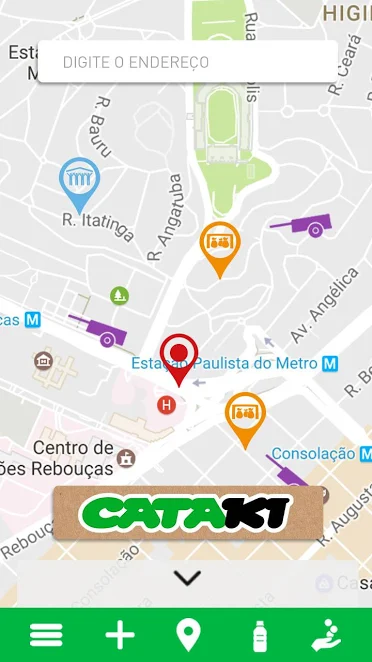
\includegraphics[scale=0.45]{media/catakimap.png}
    \legend{Fonte: Google Play}
     \label{fig:figura1}
  \end{minipage}
  \hfill
  \begin{minipage}{0.45\textwidth}
    \centering
    \caption{Cataki - Catador}
    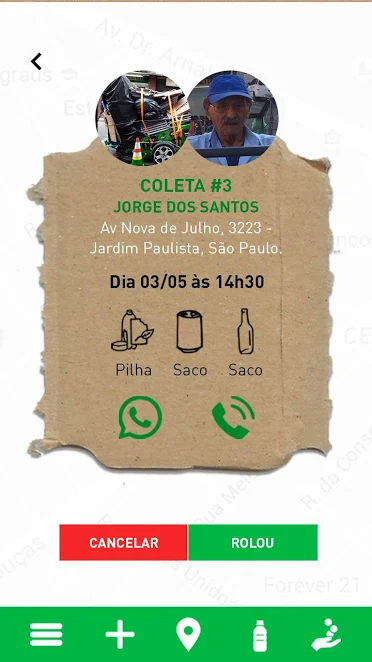
\includegraphics[scale=0.45]{media/infocatador.png}
    \legend{Fonte: Google Play}
     \label{fig:figura2}
  \end{minipage}
\end{figure}

\newpage
O Cataki também possui um banco de dados com informações genéricas sobre o descarte e sobre os materiais. A \autoref{fig:figura3} mostra os materiais disponíveis no aplicativo. Quando uma material é selecionado, uma nova tela se abre mostrando os detalhes sobre o mesmo, como mostrado na \autoref{fig:figura4}. \\
     \begin{figure}[htb]    
 \centering
  \begin{minipage}{0.45\textwidth}
    \centering
    \caption{Cataki - Materiais}
    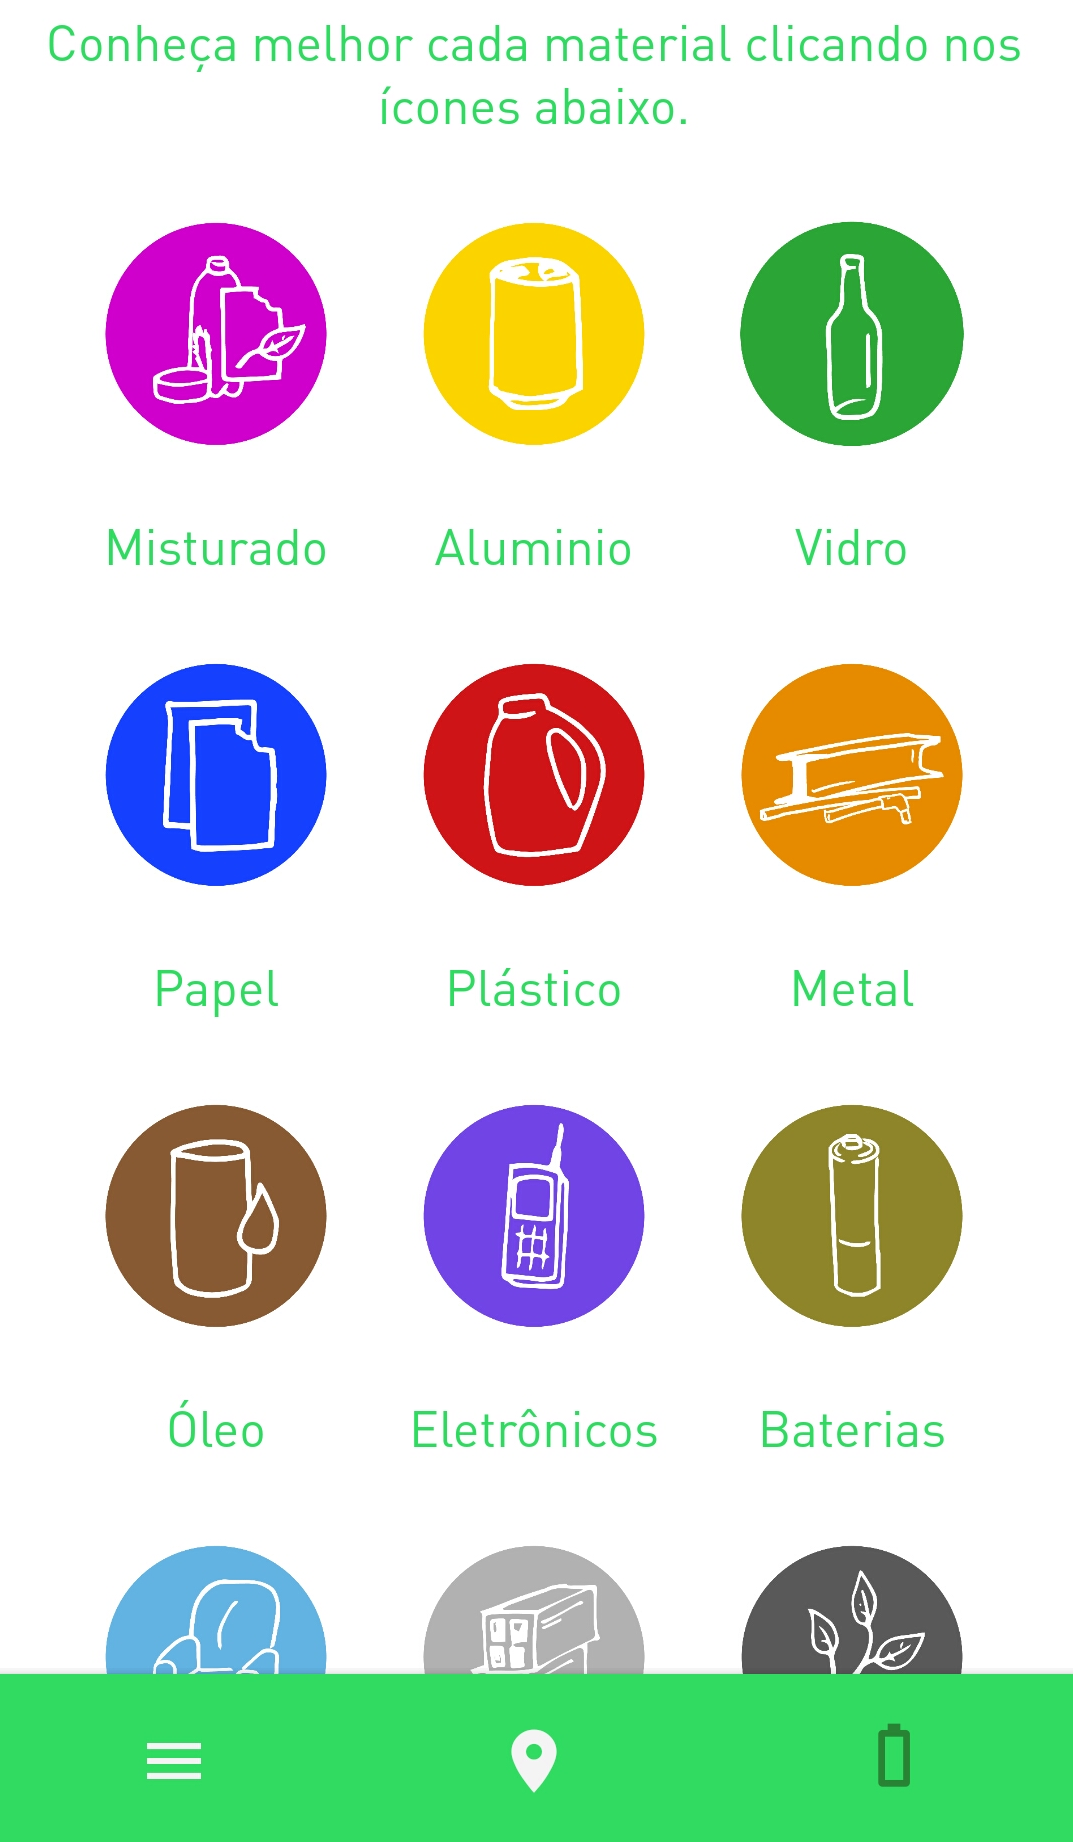
\includegraphics[scale=0.15]{media/catakimateriais.png}   
    \legend{Fonte: Google Play}
     \label{fig:figura3}
  \end{minipage}
  \hfill
  \begin{minipage}{0.45\textwidth}
    \centering
    \caption{Cataki - Detalhes}
    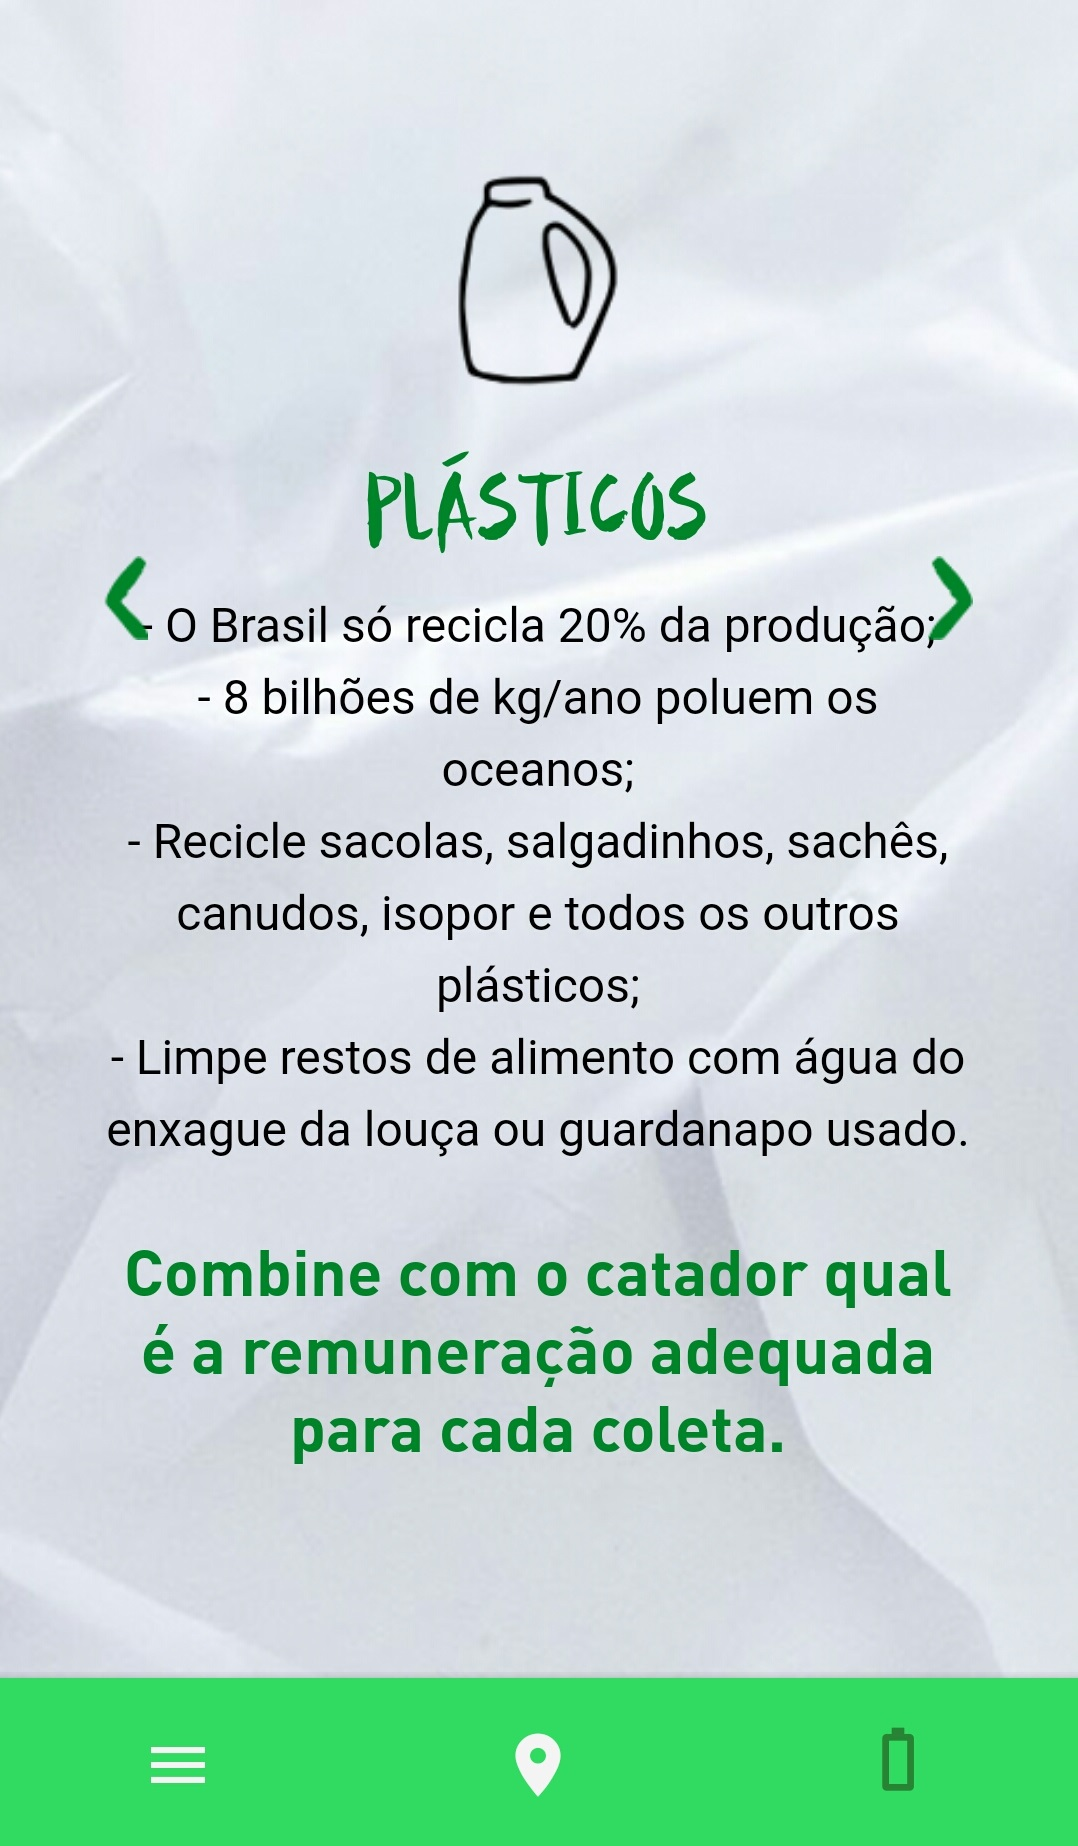
\includegraphics[scale=0.15]{media/catakimateriaisdetalhes.jpg}
    \legend{Fonte: Google Play}
     \label{fig:figura4}
  \end{minipage}
\end{figure}

\section{Recicloteca}

A Recicloteca é um centro de informações sobre reciclagem e meio ambiente criado pela ONG Ecomarapendi. Foi desenvolvido com o objetivo de difundir informações sobre as questões ambientais, com ênfase na redução, reaproveitamento e reciclagem de resíduos. Seu acervo é composto pelos mais diversos materiais, incluindo livros, vídeos, revistas, periódicos técnico-científicos, cartilhas, teses, produtos reciclados e outros.

Para utilizar a Recicloteca é preciso acessar a \footnote{http://www.recicloteca.org.br/}{página} na internet. Ao acessar a página uma das sessões relevantes para esse trabalho é a sessão de \href{http://www.recicloteca.org.br/pesquisa/}{Pesquisa Escolar} que aparece na página principal, como mostrado na \autoref{fig:reciclotecahome}.

\begin{figure}[h]
\centering
   \caption{Recicloteca - Página Inicial}
   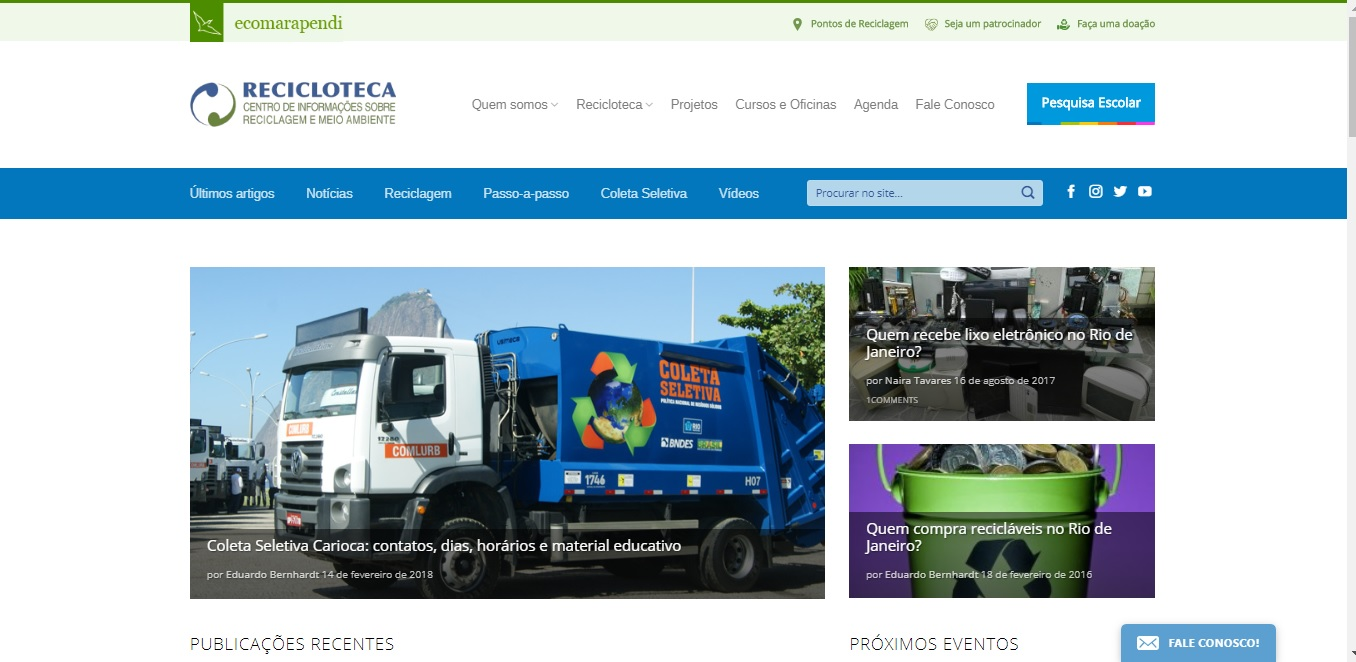
\includegraphics[scale=0.40]{media/reciclotecahome.jpg}
   \legend{Fonte: Recicloteca.org.br}
     \label{fig:reciclotecahome}
\end{figure}

Ao clicar em pesquisa escolar, o usuário é redirecionado para uma página que contém uma série de vídeos animados separados por diversas categorias, como mostra a \autoref{fig:reciclotecaescola}. Esses vídeos são feitos com uma linguagem fácil e uma animação que mantêm o interesse das crianças.

\begin{figure}[h]
\centering
   \caption{Recicloteca - Pesquisa Escolar}
   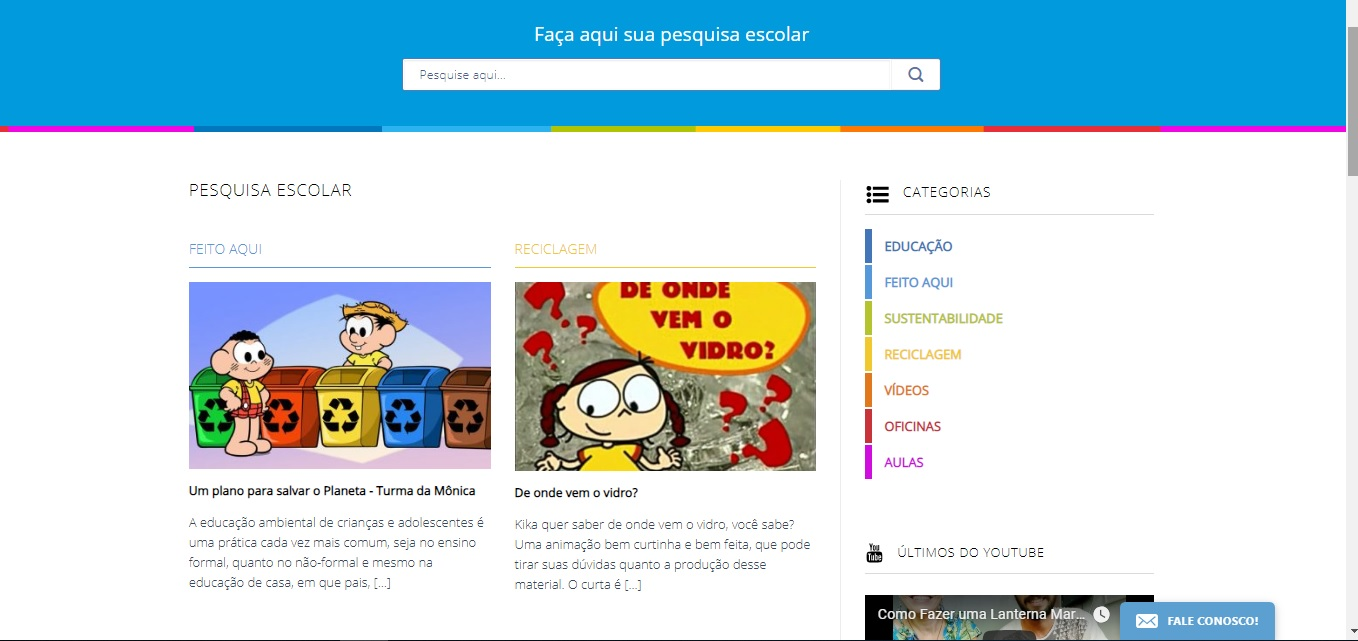
\includegraphics[scale=0.40]{media/reciclotecaescola.jpg}
   \legend{Fonte: Recicloteca.org.br}
     \label{fig:reciclotecaescola}
\end{figure}

\newpage
Outra sessão relevante para esse projeto é a \textbf{passo a passo} que pode ser acessada no menu da página principal, como mostra a \autoref{fig:reciclotecareciclagem}. Esta sessão contém vídeos e artigos ensinando como reaproveitar itens que seriam descartados, dando origem a um novo produto ou a uma nova matéria-prima, com o objetivo de diminuir a produção de rejeitos e o seu acúmulo na natureza.


\begin{figure}[h]
\centering
   \caption{Recicloteca - Passo-a-passo}
   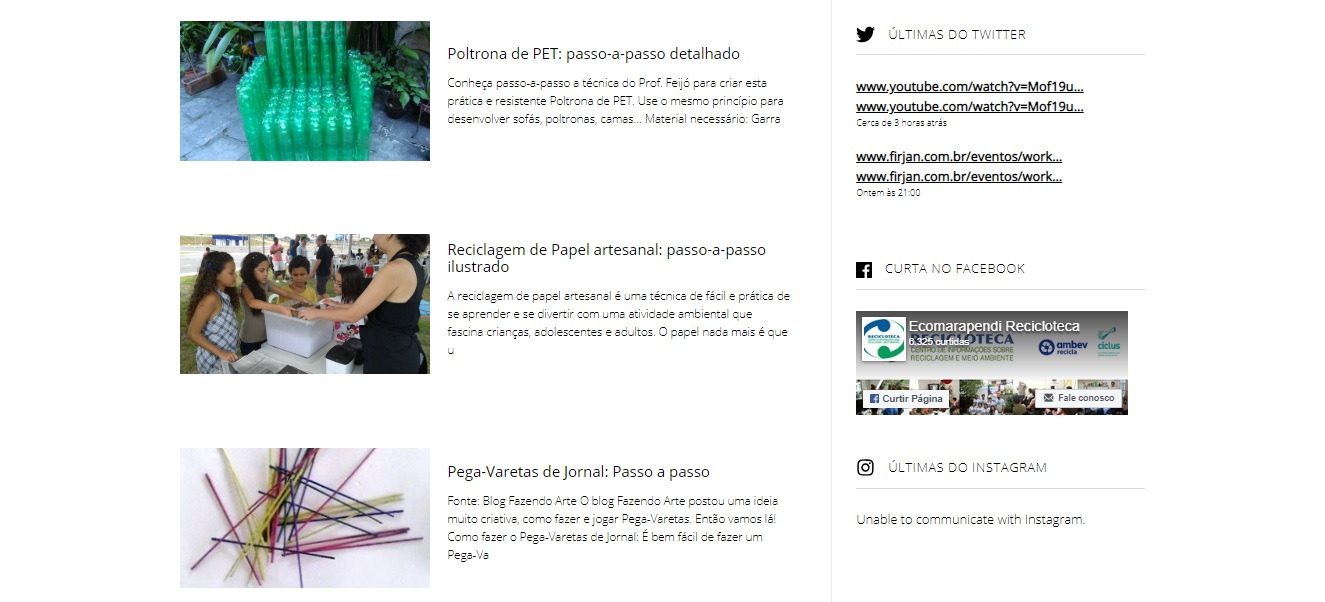
\includegraphics[scale=0.45]{media/reciclotecareciclagem.jpg}
   \legend{Fonte: Recicloteca.org.br}
     \label{fig:reciclotecareciclagem}
\end{figure}


% ---

\newpage
\section{Rota da Reciclagem}

O aplicativo Rota da Reciclagem promove a reciclagem e a defesa do meio ambiente. A \autoref{fig:rota1} mostra como qualquer pessoa interessada pode participar da separação e entrega das embalagens longa vida para a reciclagem, informando ainda onde estão localizadas as cooperativas de catadores, as empresas comerciais que trabalham com compra de materiais recicláveis e os pontos de entrega voluntária que recebem embalagens da Tetra Pak\cite{rotareciclagem}.

Para utilizar o aplicativo é preciso efetuar a transferência na Google Play ou na App Store. Após a transferência basta abrir o aplicativo que ele apresentará a tela de carregamento. Após o carregamento dos dados, uma tela com um campo de texto para inserir o endereço da sua localização aparecerá e ao ser preenchido exibirá um mapa mostrando marcadores que representam cooperativas, pontos de entrega, comércios e sua localização atual, como mostra a \autoref{fig:rota2}.
    
    

    
\begin{figure}[htb]    
 \centering
  \begin{minipage}{0.45\textwidth}
    \centering
    \caption{Rota da reciclagem - Tela de carregamento}
    
\includegraphics[scale=0.45]{media/rotaappintro.jpg}   
    \legend{Fonte: Google Play}
     \label{fig:rota1}
  \end{minipage}
  \hfill
  \begin{minipage}{0.45\textwidth}
    \centering
    \caption{Rota da reciclagem - Mapa}
    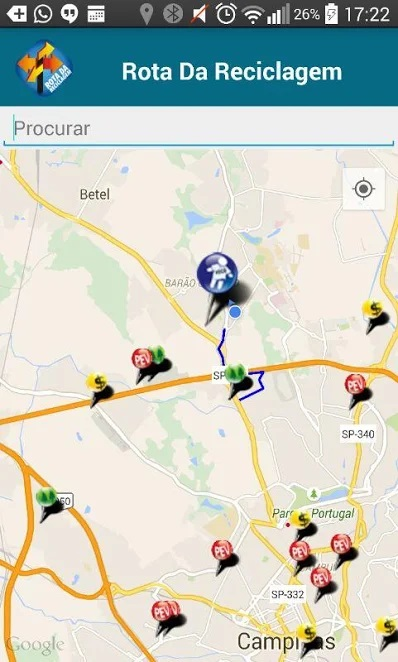
\includegraphics[scale=0.45]{media/rotaappmap.jpg}
    \legend{Fonte: Google Play}
     \label{fig:rota2}
  \end{minipage}
\end{figure}




% ----------------------------------------------------------
\begin{chapter}{Referencial Teórico}
% ----------------------------------------------------------
Neste capítulo serão apresentadas as principais características referentes ao sistema operacional Android e ao desenvolvimento de aplicativos \textit{mobile}.
\section{Desenvolvimento \textit{Mobile}}
Existem diversas plataformas de sistemas operacionais \textit{mobile} em uso nos \textit{smartphones} atuais. Grande parte desse mercado é dominado pelas plataformas Android e iOS, como mostra a \autoref{fig:plataformas_mobile}. Neste projeto utilizamos a plataforma Android devido a sua alta taxa de adesão e o pouco tempo hábil para o desenvolvimento em outras plataformas.

\begin{figure}[h]
\centering
   \caption{Divisão das plataformas mobile}
   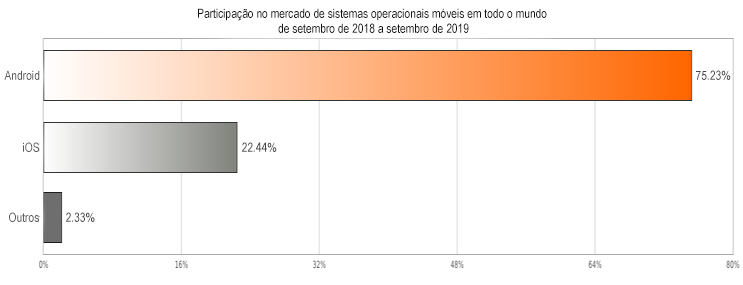
\includegraphics[scale=0.85]{media/grafico_plataformas2.png}
   \legend{Fonte: gs.statcounter.com}
     \label{fig:plataformas_mobile}
\end{figure}

\newpage
\section{SDK}
Nessa sessão serão indicados os principais \textit{Software Development Kit} (SDK) envolvidos no desenvolvimento de aplicativos Android nativo.

\begin{itemize}
\item{Android SDK} \\
O \textit{kit} de desenvolvimento de \textit{software} Android (Android SDK) é um pacote com diversas ferramentas e tecnologias utilizadas pelos desenvolvedores parar criar aplicativos para plataforma Android de forma nativa. o SDK inclui as principais bibliotecas, emuladores e ofuscadores.
  
     \item{Java SDK} \\
O \textit{kit} de desenvolvimento de \textit{software} Java (JDK) é um conjunto de utilitários e tecnologias que permitem o desenvolvimento de programas capazes de rodar em uma máquina virtual Java (JVM).
\end{itemize}


\section{Android O.S}
O Google em parceria com outras empresas lançaram o desafio de criar um plataforma móvel, na qual todos os participantes da aliança pudessem utilizar em seus \textit{hardwares} e que fosse de acesso economicamente viável à população, tirando o peso do custo de desenvolvimento de um sistema móvel completo. Assim nasceu o Android, uma pilha de \textit{softwares} para dispositivos móveis que inclui um sistema operacional, um \textit{middleware} e um conjunto de aplicações chaves. Os desenvolvedores podem criar aplicações para a plataforma usando o Android SDK (\textit{Software Development Kit}), uma IDE (\textit{Integrated Development Environment}) e uma linguagem suportada pela SDK. As aplicações para essa plataforma são comumente escritas usando a linguagem de programação Java ou Kotlin. \cite{rbhag}

Os aplicativos gerados são executados sobre o Dalvik ou ART,  máquinas virtuais customizadas para dispositivos com restrições de recursos, como pouca capacidade computacional, baixa capacidade de armazenamento e baterias com baixo nível de energia. Portanto, tais restrições devem fazer parte do projeto.

\newpage
\subsection{Arquitetura}
A arquitetura do sistema operacional Android é dividida em camadas, onde cada camada é responsável por gerenciar os seus processos. O diagrama na \autoref{fig:arquitetura} mostra essa divisão.

\begin{figure}[h]
\centering
   \caption{Arquitetura Android}
   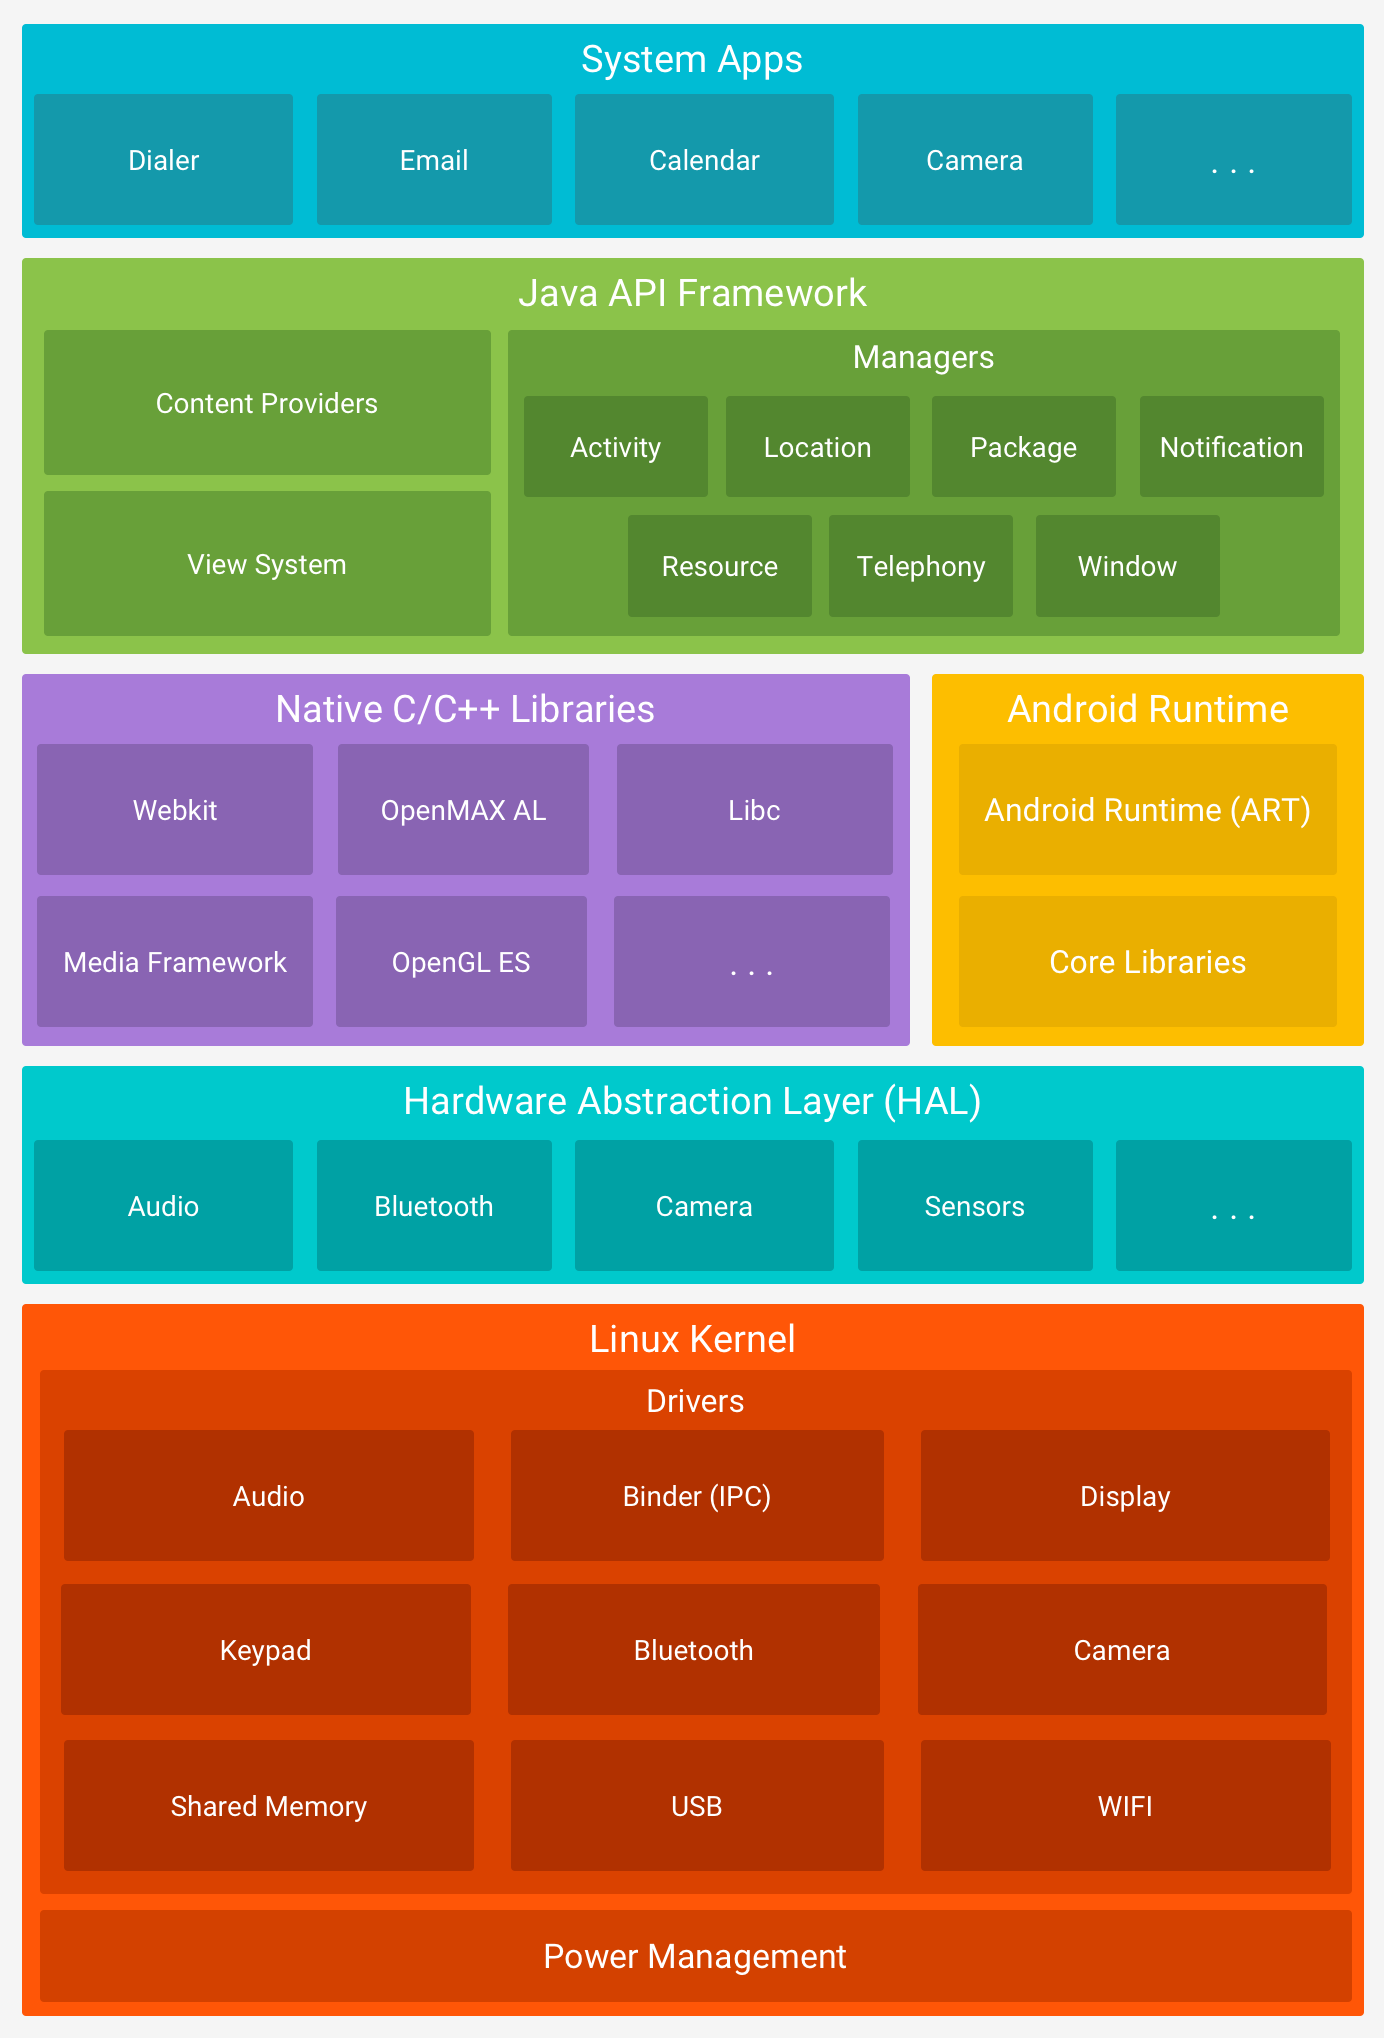
\includegraphics[scale=0.25]{media/android-stack_2x.png}
   \legend{Fonte: developer.android.com}
     \label{fig:arquitetura}
\end{figure}

\newpage

\subsubsection{Kernel}
Os dispositivos móveis possuem arquiteturas distintas e para isso é necessária uma camada capaz de gerenciar os recursos do sistema, além de fornecer aos programas do usuário uma \textit{interface} simplificada com o \textit{hardware}.
O sistema operacional Android utiliza o \textit{kernel} do Linux, que é responsável por gerenciar serviços como segurança, gerenciamento de memória, processos, rede e \textit{drivers}.

\subsubsection{Android Runtime}
O Android Runtime (ART) é um processo responsável pela compilação de códigos de alto nível (DEX bytecode) em códigos de máquina.
O processo usa uma técnica de compilação chamada AOT (\textit{Ahead of Time}). Sua principal diferença em relação ao Dalvik é que ela ocorre antes 
da execução do aplicativo e não durante a execução. Com isso, há um aumento na velocidade de execução ao custo de um processo que ocupa mais memória.



\subsubsection{Native C/C++ Libraries}
Vários componentes e diversos serviços do sistema operacional Android são implementados em código nativo,
 o que exige bibliotecas nativas desenvolvidas em C e C++.
O \textit{framework} Android oferece uma camada de abstração chamada de HAL (\textit{Hardware abstraction layer}) para expor as funcionalidades de algumas dessas bibliotecas.
Tal abstração permite a manipulação de vídeos, imagens, sons, animações, GPS, etc.

\subsubsection{Java API Framework}
Além das bibliotecas os desenvolvedores tem a sua disposição um conjunto completo de APIs na linguagem java que permitem a interoperabilidade entre aplicativos e subsistemas Android. Logo, essas APIs são a base para desenvolvimento de aplicativos Android, facilitando o acesso aos serviços do sistema como gerenciadores de janela, telefone e provedores de conteúdo.

\subsection{Componentes Android}
\subsubsection{Activity}  \label{activity}
É um componente que fornece uma tela a qual o usuário pode interagir. Um aplicativo pode ter várias activities de entrada que podem chamar inúmeras activities dependendo da interação do usuário. Para usá-las de forma correta, é necessário entender conceitos como seu ciclo de vida, gerenciamento na memória e seus métodos. 

\subsubsection{\nameref{fig:fragments_preview}} \label{fragment} 
Esse componente permite a criação de interfaces ou módulos de interface reutilizáveis e auto-gerenciáveis. esse componente só existe dentro de uma \textit{activity}. Logo, apesar de possuir seu próprio ciclo de vida, alterações no ciclo da vida da \textit{activity} afetam o ciclo de vida do \textit{fragment}.  

\begin{figure}[h]
\centering
   \caption{Fragment}
   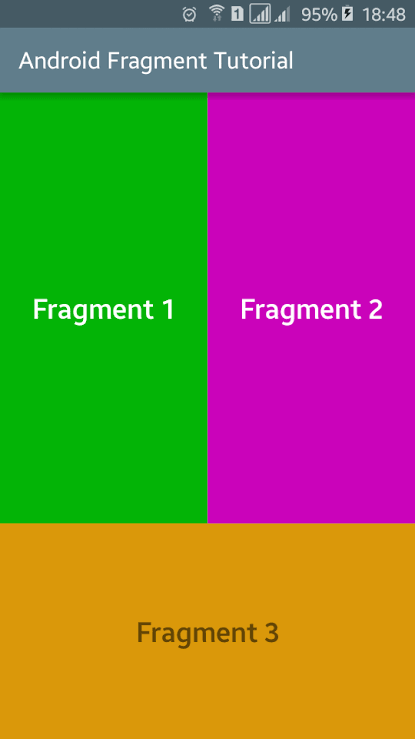
\includegraphics[scale=0.4]{media/fragments.png}
   \legend{Fonte: www.viralandroid.com}
     \label{fig:fragments_preview}
\end{figure}

\subsubsection{Intent} \label{Intent}
O \textit{Intent} é um componente do SDK Android que permite a comunicação entre outros componentes, descrevendo como o mesmo será iniciado e que dados serão recebidos durante a inicialização. O \textit{intent} é comumente utilizado para inicializar uma \nameref{activity}.

\subsubsection{Bundle} \label{Bundle}
O \textit{Bundle} é uma estrutura de chave e valor utilizada para passar valores entre \nameref{activity} e \nameref{fragment}.


\newpage
\subsubsection{\nameref{fig:viewpager}} \label{ViewPager}
\textit{ViewPager} é um gerenciador de tela que permite o usuário navegar para esquerda e para direita através de páginas de dados.
\begin{figure}[h]
\centering
   \caption{ViewPager}
   
\includegraphics[scale=0.8]{media/viewpager.jpg}
   \legend{Fonte: webheavens.com}
     \label{fig:viewpager}
\end{figure}

\subsection{\nameref{fig:tabs}} \label{TabLayout}
\textit{TabLayout} é um componente de interface gráfica  implementado junto com o \nameref{ViewPager} que permite que o usuário troque rapidamente entre as páginas.
\begin{figure}[h]
\centering
   \caption{TabLayout}
   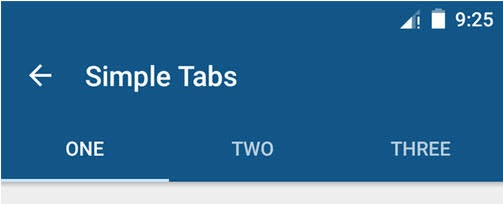
\includegraphics[scale=0.5]{media/tabs.jpg}
   \legend{Fonte: Autor}
     \label{fig:tabs}
\end{figure}

\subsubsection{\nameref{fig:recyclerview}} \label{RecyclerView}
\textit{RecyclerView} é um componente que permite a exibição de listas com alta performance utilizando a reciclagem das células da lista. Essa célula é conhecida como \textit{ViewHolder}. A construção de cada célula é feita através da implementação da classe abstrata \textit{RecyclerView.Adapter}.



\begin{figure}[h]
\centering
   \caption{RecyclerView}
   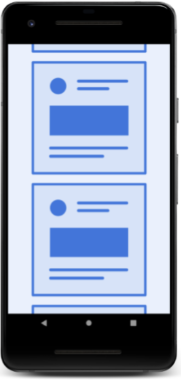
\includegraphics[scale=1.0]{media/recyclerview.png}
   \legend{Fonte: developers.google.com}
     \label{fig:recyclerview}
\end{figure}

\subsubsection{WebView} \label{WebView}
\textit{WebView} é um componente pré-instalado no sistema operacional Android que permite que os aplicativos exibam conteúdo de páginas web.

\subsubsection{MapView} \label{MapView}
É um componente que permite exibir um mapa com dados obtidos do serviço da Google, é possível adicionar marcadores no mapa destacando a região ou local desejado.


\newpage
\subsection{Gerenciamento de memória}
Em aplicativos móveis os recursos do sistema são fatores importantes para garantir o desempenho de todas as aplicações. Por isso, o sistema operacional \textit{Android} controla como seus recursos serão distribuídos. Aplicativos que estão abertos em segundo plano ou \textit{activities} empilhadas podem ter telas destruídas e variáveis removidas da memória a qualquer momento. Para solucionar esse problema o sistema operacional oferece um conjunto de \textit{callbacks} nos componentes que possuem ciclos de vida, como \nameref{activity} e \nameref{fragment}, para que o desenvolvedor possa controlar os comportamentos durante as mudanças de estado do sistema. A \autoref{fig:backstack} demonstra o processo de empilhamento durante a criação e destruição de várias \textit{activities}.

\begin{figure}[h]
\centering
   \caption{Empilhamento de activities}
   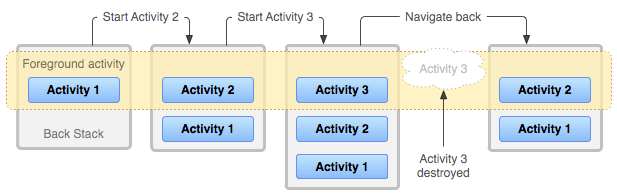
\includegraphics[scale=0.70]{media/diagram_backstack.png}
   \legend{Fonte: developer.android.com}
     \label{fig:backstack}
\end{figure}

\subsection{Ciclo de vida}
À medida que o usuário navega no aplicativo, sai dele e retorna a ele, as instâncias \nameref{activity} no aplicativo transitam entre diferentes estados no \nameref{fig:lifecycle}. A classe \textit{activity} fornece uma quantidade de \textit{callbacks} que permite que o desenvolvedor saiba sobre a mudança do estado.

O Diagrama a seguir mostra quando os \textit{callback} são executados durante a mudança do ciclo de vida da \textit{activity}.
\begin{figure}[h]
\centering
   \caption{Ciclo de vida}
   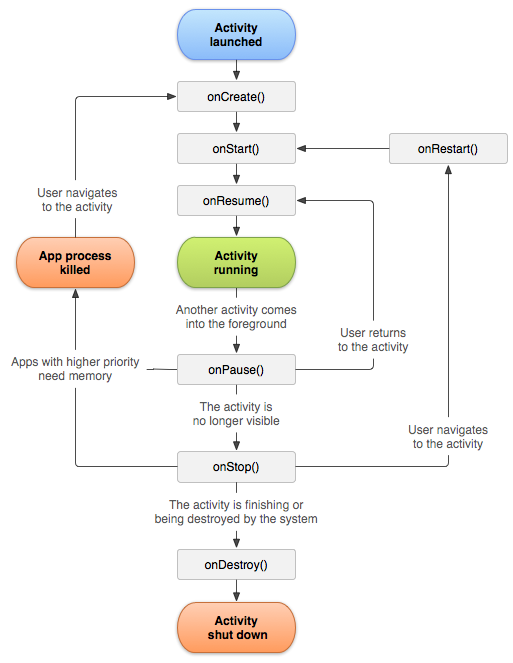
\includegraphics[scale=0.70]{media/activity_lifecycle.png}
   \legend{Fonte: developer.android.com}
     \label{fig:lifecycle}
\end{figure}

\newpage
\begin{itemize}
\item{OnCreate} \\
     É chamado assim que uma \nameref{activity} ou \nameref{fragment} é iniciado, boa parte da inicialização é feita nesse \textit{callback}, incluindo o processo de criação da interface de usuário. O \textit{onCreate} é executado uma vez durante a inicialização e só será chamado novamente caso o sistema operacional decida destruir a \textit{activity}, para liberar recursos para uma \textit{activity} com maior prioridade.
     
     \newpage
     \item{OnStart} \\
     Chamado após o \textit{OnCreate} ou após o \textit{OnRestart}, o \textit{Onstart} é executado quando a interface gráfica está visível, porem o usuário ainda não pode interagir. Esse \textit{callback} é normalmente utilizado inicializações adicionais, desenhar componentes e executar animações.
     \item{OnResume} \\
      Chamado quando a atividade vai iniciar a interação com o usuário. Nesse ponto, sua atividade está no topo da pilha de atividades. 
      \item{OnRestart} \\
      Chamada após o \textit{OnStop} quando uma \textit{activity} que está na pilha é recriada. 
     \item{OnPause} \\
     Chamado quando o sistema está por resumir a \textit{activity} anterior. É tipicamente usado para persistir mudanças ainda não efetivadas, parar animações e liberar recursos. A partir desse ponto o sistema operacional pode forçar a liberação de recursos consumidos pela \textit{activity} pausada. 
     \item{OnStop} \\
    Chamado quando a \textit{activity} não está mais visível para o usuário. Isso pode acontecer porque ela está sendo destruída ou porque outra  \textit{activity} foi reiniciada e está em sua frente. Aqui é o lugar para liberar todos os recursos que não são mais utilizados pelo usuário. 
     \item{OnDestroy} \\
     Chamado quando a \textit{activity} vai ser destruída. É a última chamada que a \textit{activity} receberá antes de ser finalizada.
  \end{itemize}

\section{API} \label{API}
A \textit{Application Programming Interface} (API) permite a comunicação e consumo de dados entre aplicações. Um dos motivos que tornam o uso de uma \textit{API} atrativo é a abstração, já que não é necessário conhecer a plataforma ou maneira que o aplicativo consumidor foi desenvolvido. Outra vantagem é o fato deste modelo ser baseado em tecnologias padrões, em particular o HTTP (Hypertext Transfer Protocol). Os dados transferidos entres essas aplicações seguem um formato padrão. Os mais utilizados são \textit{JavaScript Object Notation} (\nameref{JSON}) e \textit{Extensible Markup Language} (XML). Neste projeto utilizamos JSON para coletar as informações como localização e tipos de materiais da API.

\newpage
\section{JSON} \label{JSON}
\textit{JavaScript Object Notation} (JSON) é um formato leve de troca de dados entre sistemas independente de linguagem de programação. O formato foi derivado do JavaScript, sendo fácil para humanos ler e escrever. O texto abaixo representa um objeto no formato JSON.

\begin{lstlisting}
{
   "Pessoa":{
      "nome": "Flávio",
      "sobrenome": "Telles"
   }
}
\end{lstlisting}

\section{Firebase}
\subsection{Firebase Realtime Database} \label{Firebase Realtime Database}
O \footnote{https://firebase.google.com/}{\textit{Firebase Realtime Database}} é um banco de dados hospedado na nuvem. Com ele é possível armazenar os dados em um formato \nameref{JSON} e sincronizar dados entre os seus usuários em tempo real, permitindo que os dados continuem disponíveis quando o aplicativo estiver \textit{off-line}.

\subsection{Firebase Authentication}
O objetivo do \textit{Firebase Authentication} é facilitar o desenvolvimento de um sistema de autenticação seguro e melhorar a experiência de \textit{login} e ambientação para os usuários finais. Ele oferece uma solução de identidade completa, compatível com contas de e-mail/senha, autenticação por telefone, \textit{login} do Google, Twitter, Facebook, GitHub e outros.
\end{chapter}
\begin{chapter}{Projeto}
Neste capítulo serão apresentadas as instalações e configurações iniciais das ferramentas e bibliotecas utilizadas no desenvolvimento de aplicativos Android.
\section{Instalação} Nesta seção serão abordados os recursos necessários para iniciar o desenvolvimento desse projeto.
\begin{enumerate}
  \item{Android Studio} \\
  Neste projeto utilizamos o Android Studio, a IDE recomendada pela Google para o desenvolvimento de aplicativos nativos. O Android Studio está disponível em \url{https://developer.android.com/studio/install}.
  \item{SDK e JDK} \\ Para iniciar o desenvolvimento Android foi instalado o Android SDK, que por sua vez necessita do JDK, já que o código gerado pelo SDK roda em uma máquina virtual Java customizada, a ART.
  O JDK esta disponível em \url{https://www.oracle.com/technetwork/java/javase/downloads/index.html} e o SDK em \url{https://developer.android.com/studio}.
  \item{GIT} \\
  Para realizar o controle de versão do aplicativo usamos o GIT, um sistema de controle de versões distribuído, usado principalmente no desenvolvimento de \textit{software}, mas pode ser usado para registrar o histórico de edições de qualquer tipo de arquivo. 
  GIT está disponível em \url{https://www.git-scm.com/}.
  
\end{enumerate}



\section{Configuração}
\subsection{Gradle}
Gradle é um sistema de automação de compilação de código aberto utilizado para configuração de projetos. Foi projetado para suportar \textit{builds}\footnote{Processo de compilação de um programa} incrementais e determinar que partes do projeto precisam ser atualizadas, atualizando somente as dependências necessárias.
No projeto Android, o arquivo de configuração do Gradle pode ser encontrado no diretório abaixo. \begin{lstlisting}[
    basicstyle=\small,
]
/app/build.gradle
\end{lstlisting}
\subsection{Dependências}
 No build.gradle, o campo \textit{dependencies} nos permite baixar bibliotecas externas, adicionar arquivos jar ou módulos em nosso projeto Android. Neste projeto utilizamos as seguintes dependências:
 
 
   \begin{itemize}
  \item{Google Play Services} \\
     As bibliotecas criadas pela Google disponíveis em \url{https://developers.google.com/android/guides/setup}, oferecem aos desenvolvedores os últimos recursos e funcionalidades mantidas pela Google, como por exemplo, GPS e mapas.
       \begin{lstlisting}[
    basicstyle=\small,
] 
implementation 'com.google.android.gms:play-services-maps:15.0.1'
implementation 'com.google.android.gms:play-services-location:15.0.1'
implementation 'com.google.android.gms:play-services-places:15.0.1'
\end{lstlisting}
\item{Volley} \\
   Também desenvolvida pela Google, disponível em \url{https://github.com/google/volley}, Volley é uma biblioteca que permite realizar requisições HTTP de forma simplificada, sem a necessidade de criação de chamadas assíncronas.
       \begin{lstlisting}[
    basicstyle=\small,
]
implementation 'com.android.volley:volley:1.1.0'  
\end{lstlisting}
\item{Lottie}

  Lottie disponível em \url{https://github.com/airbnb/lottie-android} é uma  biblioteca que simplifica a criação de animações complexas exportando animações profissionais em formato \nameref{JSON}.
        \begin{lstlisting}[
    basicstyle=\small,
] 
implementation 'com.airbnb.android:lottie:$lottieVersion'
\end{lstlisting}
\item{MPAndroidChart} \\
   A  MPAndoridChart disponível em \url{https://github.com/PhilJay/MPAndroidChart} é uma poderosa biblioteca que simplifica a criação de diversos tipos de gráficos. 
        \begin{lstlisting}[
    basicstyle=\small,
] 
implementation 'com.github.PhilJay:MPAndroidChart:v3.0.3'
  
\end{lstlisting}
\item{Firebase} \\
O Firebase, disponível em \url{https://firebase.google.com} é um conjunto de soluções criadas pela Google para agilizar e melhorar o desenvolvimento de aplicações. Neste projeto usamos somente o \textit{Firebase Realtime Database}, que é um banco de dados hospedado na nuvem. Os dados são armazenados como \nameref{JSON} e sincronizados em tempo real com todos os clientes conectados
        \begin{lstlisting}[
    basicstyle=\small,
]
implementation 'com.google.firebase:firebase-database:16.0.1'
  
\end{lstlisting}
\item{Glide} \\
   disponível em \url{https://github.com/bumptech/glide}, Glide é uma biblioteca de gerenciamento e carregamento de imagens 
que simplifica tarefas como decodificação, cache em memória e em disco. 
        \begin{lstlisting}[
    basicstyle=\small,
]
implementation 'com.github.bumptech.glide:glide:4.7.1'
  
\end{lstlisting}
\item{SmartTabLayout} \\
 A biblioteca SmartTabLayout disponível em \url{https://github.com/ogaclejapan/SmartTabLayout}, fornece uma implementação mais customizável 
para criação de menus em componentes do sistema operacional Android.
         \begin{lstlisting}[
    basicstyle=\small,
]
implementation 'com.ogaclejapan.smarttablayout:library:1.6.1@aar'
   
\end{lstlisting}
        \begin{lstlisting}[
    basicstyle=\small,
]
implementation 'com.ogaclejapan.smarttablayout:utils-v4:1.6.1@aar'
   
\end{lstlisting}
\item{Gson} \\
   Desenvolvida pela Google, disponível em \url{https://github.com/google/gson}, Gson é uma biblioteca que pode ser usada para converter objetos Java (POJO) em representações \nameref{JSON} ou vice-versa.
         \begin{lstlisting}[
    basicstyle=\small,
]
implementation 'com.google.code.gson:gson:2.8.5'
    
\end{lstlisting}
\item{YouTubeAndroidPlayerApi} \\
   Desenvolvida pela Google, disponível em \url{https://developers.google.com/youtube/android/player}, YouTubeAndroidPlayerApi permite incorporar a funcionalidade de reprodução de vídeo em aplicativos Android. A API  define métodos para carregar, reproduzir 
e controlar a experiência de reprodução de vídeo.
      \begin{lstlisting}[
    basicstyle=\small,
]
implementation files('libs/YouTubeAndroidPlayerApi.jar')
   
\end{lstlisting}
\item{Fabric} \\
   A biblioteca Fabric, também conhecida como Crashlytics, disponível em \url{https://fabric.io/kits/android/crashlytics/install}, ajuda a rastrear, priorizar e corrigir problemas de instabilidade que podem prejudicar a qualidade do aplicativo e a experiência do usuário.
   \begin{lstlisting}[
    basicstyle=\small,
]
implementation 'com.crashlytics.sdk.android:crashlytics:2.9.9'
   
\end{lstlisting}
\end{itemize}

\section{Desenvolvimento}
Nesta seção, serão abordadas as etapas do desenvolvimento da solução proposta nesse documento, desde a criação do subsistema que irá gerenciar todo conteúdo até o aplicativo Android. 

\subsection{\nameref{fig:arquitetura_geral}}
Para possibilitar a entrega de conteúdo dinâmico no aplicativo, foi escolhida uma arquitetura cliente-servidor onde o aplicativo consome dados em servidores da Google através de uma API ou SDK. Esses servidores são preenchidos com informações relevantes ao aplicativo através de uma página \textit{web} administrativa hospedada nos servidores do Firebase. O processo de desenvolvimento dessa página será abstraído neste documento.\\


\begin{figure}[h]
\centering
   \caption{Arquitetura geral}
   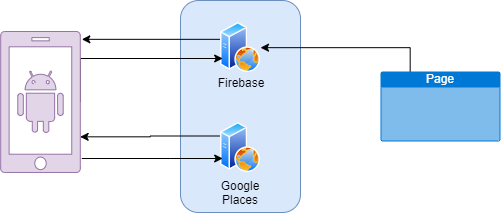
\includegraphics[scale=0.85]{media/arquitetura_app.png}
   \legend{Fonte: Autor}
     \label{fig:arquitetura_geral}
\end{figure}

\subsection{Arquitetura do Aplicativo}
Os padrões de arquitetura ajudam os desenvolvedores a desenvolver aplicativos fracamente acoplados, fáceis de testar e manter.
Neste projeto usamos \textit{Model-View-Controller} (MVC).

\subsubsection{MVC}
A arquitetura \nameref{fig:arquitetura_mvc} consiste na divisão do aplicativo em três camadas,  \textit{model}, \textit{view} e \textit{controller}. Por questões da arquitetura do sistema operacional Android e sua SDK, não é possível implementar um padrão arquitetural MVC da forma convencional, pois \textit{fragments} e \textit{activities} assumem papéis da camada \textit{controller} e \textit{view} simultaneamente.

\begin{itemize}
  \item{Model}\\ Essa camada fica responsável pelo acesso aos repositórios para salvar e entregar dados a camada controladora.
     \item{View}\\ Essa camada fica responsável pela apresentação da interface gráfica.
       \item{Controller}\\ A camada \textit{controller} é responsável por implementar as regras de negócio e fornecer os dados do modelo para a camada \textit{view}. Quaisquer alterações ao controlador são transparentes para a \textit{view} e as mudanças de interface do usuário não afetarão a lógica de negócios e vice-versa.
\end{itemize}

\begin{figure}[h]
\centering
   \caption{MVC}
   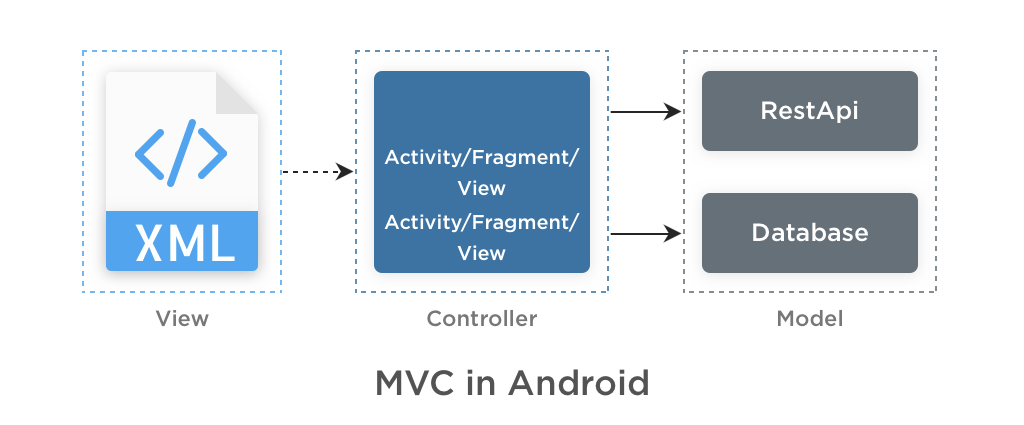
\includegraphics[scale=0.40]{media/MVC.png}
   \legend{Fonte: www.simform.com}
     \label{fig:arquitetura_mvc}
\end{figure}


\subsection{Banco de dados}
Para a persistência da dados foi escolhido o banco de dados mais popular entre os desenvolvedores mobile, o \textit{Firebase Realtime Database}. O \textit{Firebase}, através da sua SDK, oferece um desenvolvimento simplificado, facilitando processos comuns em aplicações \textit{mobile}, como autenticação, leitura e escrita de dados.
 Os diagramas a seguir representam as entidades que serão utilizadas neste projeto.


\subsubsection{Entidades}
\begin{enumerate}
 \item{Material} \\ A classe \textit{\nameref{fig:materialmodel}} representa a estrutura de um material reciclável. Por exemplo, ferro, plástico e papel. Esta classe possui os seguintes atributos:
 
 \begin{itemize}
  \item{Cod}\\ Identificador único do material.
   \item{PopularName}\\ Nome popular do material.
     \item{Name}\\ Nome cientifico do material.
       \item{Content}\\ informações detalhadas do material.
         \item{Type}\\ Tipo de material.
           \item{Image}\\ Imagem ilustrativa do material.
\end{itemize}
  
\begin{figure}[h]
\centering
   \caption{MaterialModel}
   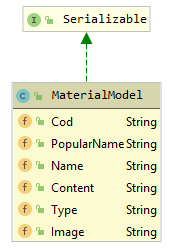
\includegraphics[scale=1.0]{media/materialModel.png}
   \legend{Fonte: Autor}
     \label{fig:materialmodel}
\end{figure}


  \item{Vídeo}  \\ A classe \textit{\nameref{fig:videomodel}} representa a estrutura de um vídeo que será disponibilizado através de uma \textit{url} do \textit{YouTube}. Esta classe possui os seguintes atributos:
   \begin{itemize}
  \item{Cod}\\ Identificador único do vídeo.
   \item{Url}\\ Endereço do vídeo no YouTube.
     \item{Title}\\ Titulo do vídeo que será apresentado no aplicativo.
       \item{Description}\\ Descrição do vídeo que será apresentado no aplicativo.
         \item{Page}\\  O identificador único da página em que será apresentado o vídeo.
\end{itemize}
  
\begin{figure}[h]
\centering
   \caption{VídeoModel}
   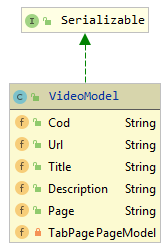
\includegraphics[scale=1.0]{media/VideoModel.png}
   \legend{Fonte: Autor}
     \label{fig:videomodel}
\end{figure}


  \item{Produto} \\ A classe \textit{\nameref{fig:productModel}} representa a estrutura de um produto. Por exemplo, telefones, brinquedos e produtos descartáveis em geral. Esta classe possui os seguintes atributos:
  
     \begin{itemize}
  \item{Cod}\\ Identificador único do produto.
     \item{Title}\\ Titulo ou nome do produto.
       \item{Desc}\\ Descrição do produto.
         \item{Synonymous}\\ Nomes alternativos do produto.
                  \item{Discard}\\ Identificador único de um tipo de descarte.
\end{itemize}
  
\begin{figure}[h]
\centering
   \caption{ProductModel}
   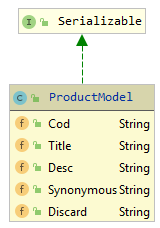
\includegraphics[scale=1.0]{media/ProductModel.png}
   \legend{Fonte: Autor}
     \label{fig:productModel}
\end{figure}

\newpage

  \item{Localização}  \\ A classe \textit{\nameref{fig:locationModel}} representa a estrutura de uma localização no mapa. Por exemplo, centros de reciclagem, lixões e aterros. Esta classe possui os seguintes atributos:
  
       \begin{itemize}
  \item{UniqueID}\\ Identificador único de uma localização.
     \item{FormattedAddress}\\ O endereço formatado de um local.
       \item{Name}\\ Nome do local.
         \item{Location}\\ Posição baseada no sistema de posicionamento global (GPS), com latitude e longitude.
\end{itemize}
  
  
\begin{figure}[h]
\centering
   \caption{LocationModel}
   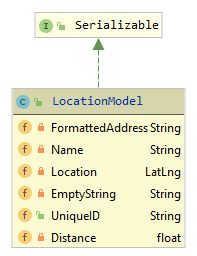
\includegraphics[scale=0.85]{media/LocationModel.png}
   \legend{Fonte: Autor}
     \label{fig:locationModel}
\end{figure}

\newpage
  \item{Gráfico}   \\ A classe \textit{\nameref{fig:chartModel}} representa a estrutura de um gráfico do tipo \textit{PieChart} ou \textit{BarChart}. Esta classe possui os seguintes atributos:
  
  \begin{itemize}
  \item{UniqueID}\\ Identificador único de um gráfico.
     \item{Data}\\ Um conjunto pré formatado de dados a serem inseridos no gráfico.
       \item{Label}\\ Etiquetas que descreve os dados apresentados no gráfico.
         \item{Type}\\ O tipo de gráfico.
         \item{Title}\\ O título do gráfico.
         \item{Page}\\  O identificador único da página em que será apresentado o gráfico.
\end{itemize}
  
\begin{figure}[h]
\centering
   \caption{ChartModel}
   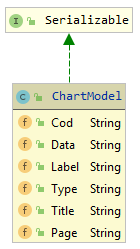
\includegraphics[scale=1.0]{media/chartModel.png}
   \legend{Fonte: Autor}
     \label{fig:chartModel}
\end{figure}


  \item{Descarte}   \\ A classe \textit{\nameref{fig:discardModel}} representa a estrutura de um método de descarte de materiais. Por exemplo, lixão, aterro e centro de reuso. Esta classe possui os seguintes atributos:
  
  \begin{itemize}
  \item{Cod}\\ Identificador único de um gráfico.
       \item{Title}\\Titulo do tipo descarte.
         \item{Desc}\\ Descrição do descarte.
  
    
\end{itemize}
  
\begin{figure}[h]
\centering
   \caption{DiscardModel}
   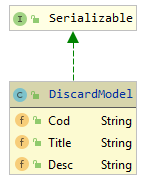
\includegraphics[scale=1.0]{media/discardModel.png}
   \legend{Fonte: Autor}
     \label{fig:discardModel}
\end{figure}

  \item{Página}   \\ A classe \textit{\nameref{fig:pageModel}} representa a estrutura de uma página que pertence a uma categoria. Esta classe possui os seguintes atributos:
  \begin{itemize}
  \item{Cod}\\ Identificador único de um gráfico.
       \item{Number}\\Número da página.
         \item{Type}\\ Categoria da página.
          \item{Type}\\ Título da página.
\end{itemize}
\begin{figure}[h]
\centering
   \caption{PageModel}
   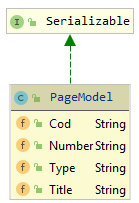
\includegraphics[scale=1.0]{media/PageModel.png}
   \legend{Fonte: Autor}
     \label{fig:pageModel}
\end{figure}

\newpage
\item{Dados Englobados}   \\ A classe \textit{\nameref{fig:datawrapper}} engloba todos os dados que serão utilizados na aplicação. Essa classe foi criada para facilitar a requisição de dados em uma única requisição ao servidor. Vale ressaltar que dados como imagens e vídeos são enviados para o aplicativo de acordo com a necessidade. Logo, não há sobrecarga ao realizar uma única requisição.
\newline
  \begin{itemize}
  \item{GraphList}\\ Todos os gráficos.
       \item{PageList}\\  Todas as páginas.
         \item{VideoList}\\ Todos os vídeos.
         \item{LocationList}\\ Todas as localizações pesquisadas pelo usuário.
         \item{ProductList}\\  Todos os produtos.
         \item{DiscardList}\\ Todos os métodos de descarte.
         \item{MaterialList}\\  Todos os materiais.
         
\end{itemize}
\begin{figure}[h]
\centering
   \caption{DataWrapper}
   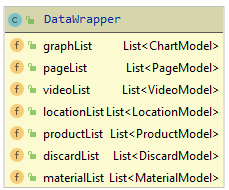
\includegraphics[scale=1.0]{media/DataWrapperModel.png}
   \legend{Fonte: Autor}
     \label{fig:datawrapper}
\end{figure}
\end{enumerate}

\newpage
\subsubsection{Diagrama de classe}
A \autoref{fig:datawrapper_simp} e \autoref{fig:datawrapper_comp} representam as dependências entre as entidades.

\begin{figure}[h]
\centering
   \caption{Diagrama - Simplificado}
   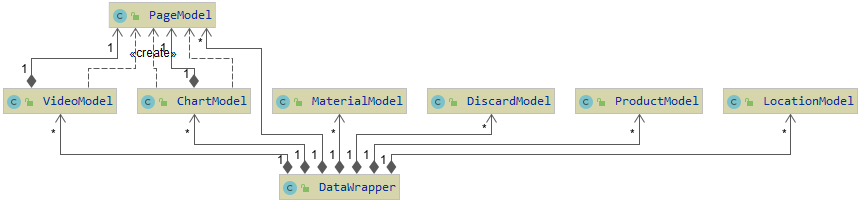
\includegraphics[scale=0.7]{media/DataWrapper_.png}
   \legend{Fonte: Autor}
     \label{fig:datawrapper_simp}
\end{figure}

\begin{figure}[h]
\centering
   \caption{Diagrama - Completo}
   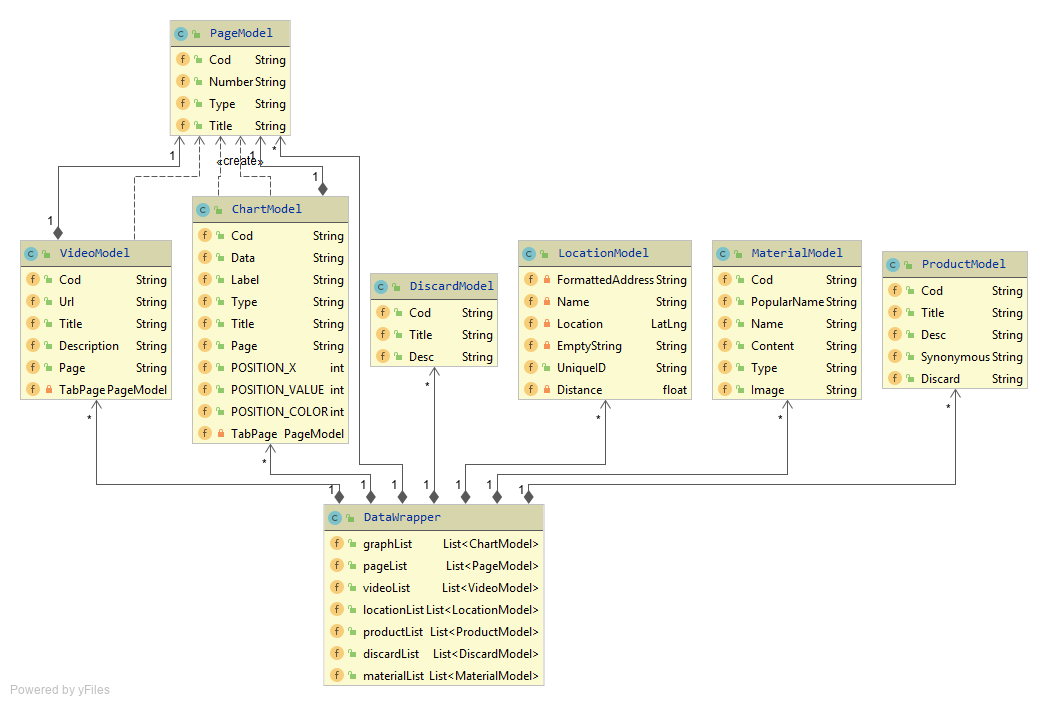
\includegraphics[scale=0.85]{media/DataWrapper.png}
   \legend{Fonte: Autor}
     \label{fig:datawrapper_comp}
\end{figure}

\newpage
\subsection{Sistema Administrativo} \label{Sistema Administrativo}
Para disponibilizar dados para o aplicativo mobile foi desenvolvido um sistema administrativo responsável por inserir ou modificar o conteúdo exibido. O sistema foi desenvolvido usando tecnologias web, como HTML, \textit{JavaScript} e CSS. Nesta seção serão abordadas as principais funcionalidades do sistema, abstraindo parte da implementação. O código fonte está disponível em \url{https://github.com/flaviotps/Reciclando_site}.

\subsubsection{\nameref{fig:tela_login_site_1}} \label{tela_auth}
Para controlar o acesso ao sistema foi desenvolvido um sistema de autenticação por e-mail utilizando o \textit{firebase authentication}. Dessa forma somente usuários cadastrados e com perfis de acesso podem realizar alterações e inclusões de conteúdo pelo sistema administrativo. 
A alteração e inclusão de novos usuários é feita diretamente pelo painel administrativo do \textit{firebase}.


\begin{figure}[h]
\centering
   \caption{Tela de autenticação}
   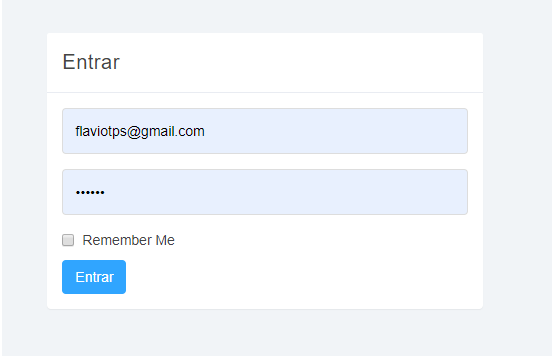
\includegraphics[scale=0.85]{media/tela_login_site_1.png}
   \legend{Fonte: Autor}
     \label{fig:tela_login_site_1}
\end{figure}

\subsubsection{Tela de materiais} \label{tela_material}
A \autoref{fig:tela_material_site_1} e \autoref{fig:tela_material_site_2} apresentam as telas que são responsáveis por inserir e modificar materiais recicláveis, como, por exemplo, plástico, metais e papéis. As informações do material podem ser escritas em HTML, tornando menu mais flexível.
\begin{figure}[h]
\centering
   \caption{Material - Todos}
   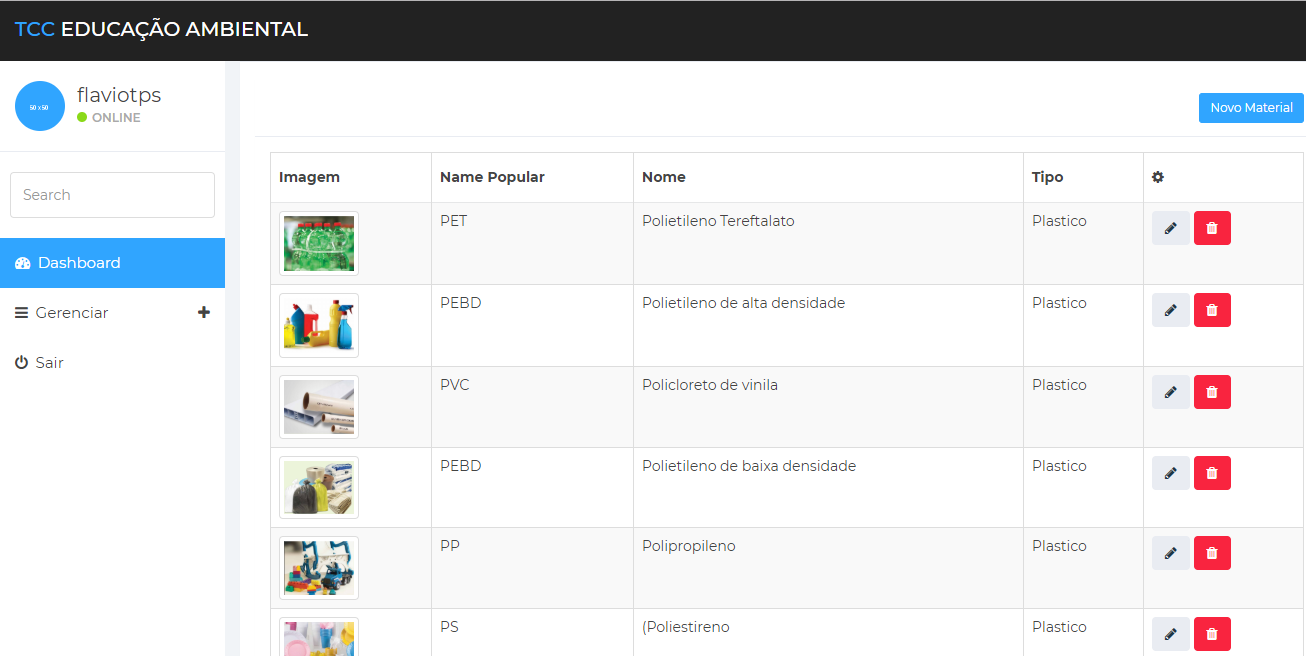
\includegraphics[scale=0.45]{media/tela_material_site_1.png}
   \legend{Fonte: Autor}
     \label{fig:tela_material_site_1}
\end{figure}

\begin{figure}[h]
\centering
   \caption{Material - Edição}
   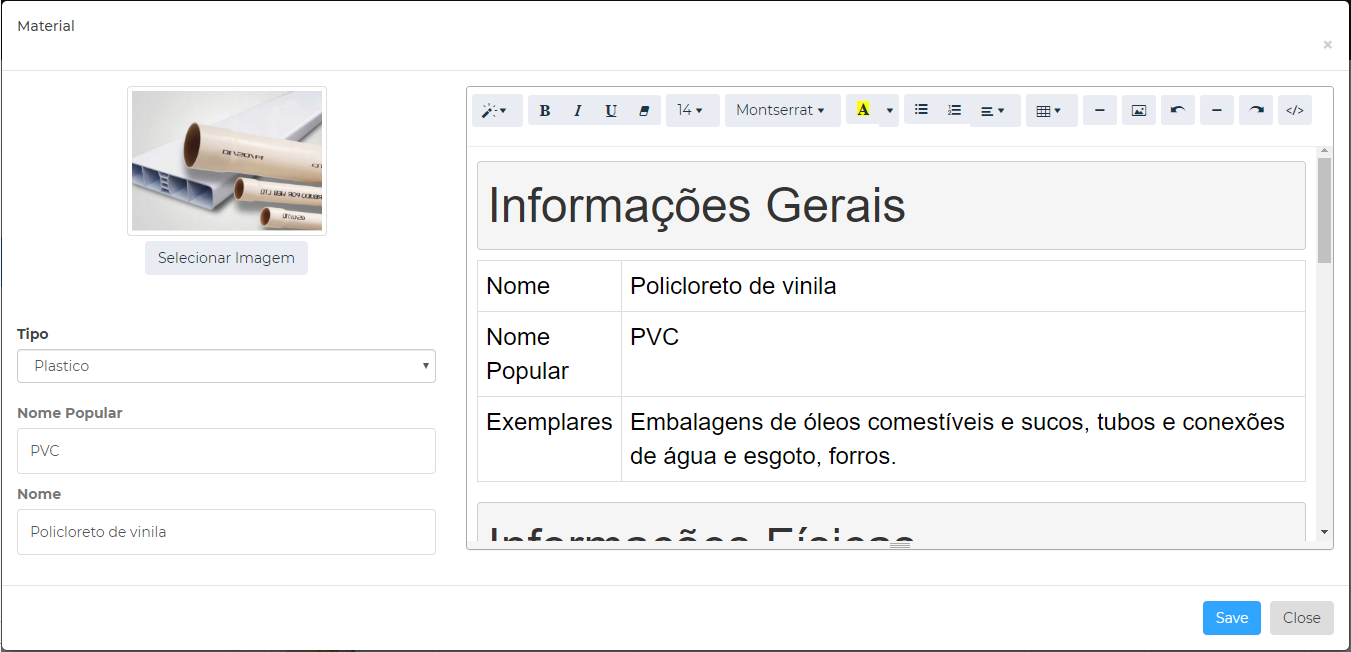
\includegraphics[scale=0.40]{media/tela_material_site_2.png}
   \legend{Fonte: Autor}
     \label{fig:tela_material_site_2}
\end{figure}

\newpage
\subsubsection{Tela de produtos} \label{tela_produtos}
A \autoref{fig:tela_produto_site_1} e \autoref{fig:tela_produto_site_2} apresentam a área que permite adicionar produtos de uso diário, como, por exemplo, telefones, brinquedos e utensílios domésticos. 

\begin{figure}[h]
\centering
   \caption{Produto - Todos}
   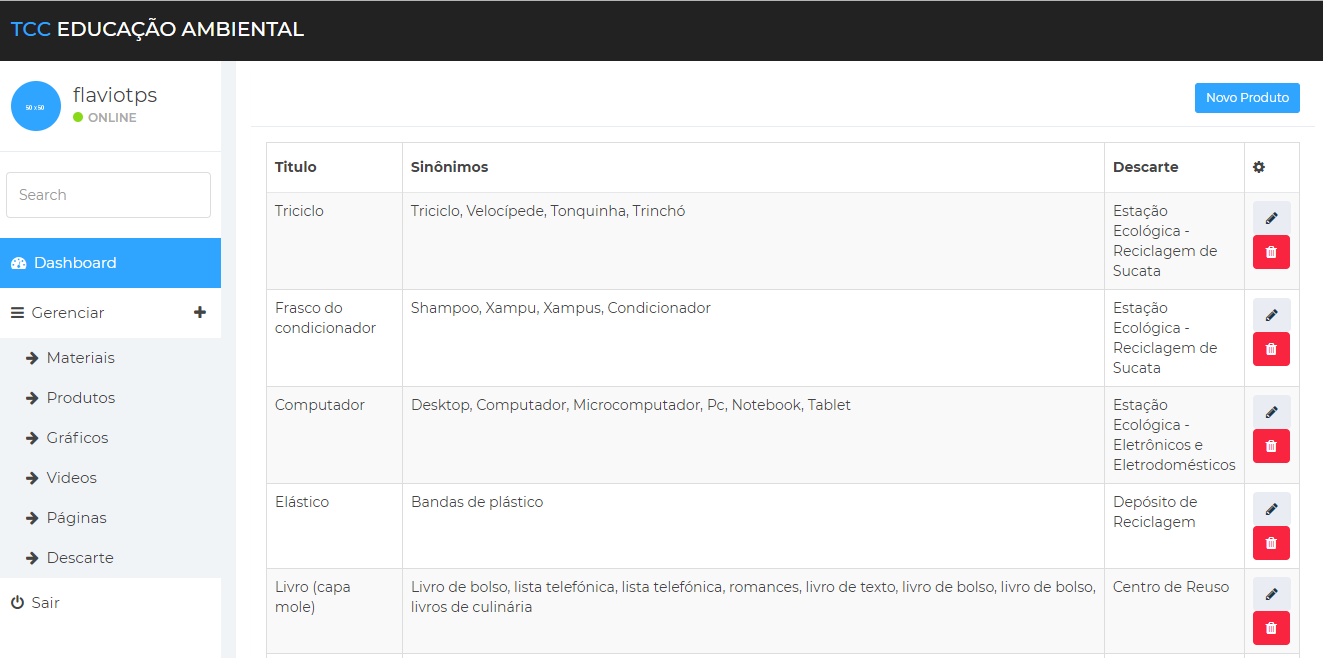
\includegraphics[scale=0.45]{media/tela_produto_site_1.png}
   \legend{Fonte: Autor}
     \label{fig:tela_produto_site_1}
\end{figure}

\begin{figure}[h]
\centering
   \caption{Produto - Edição}
   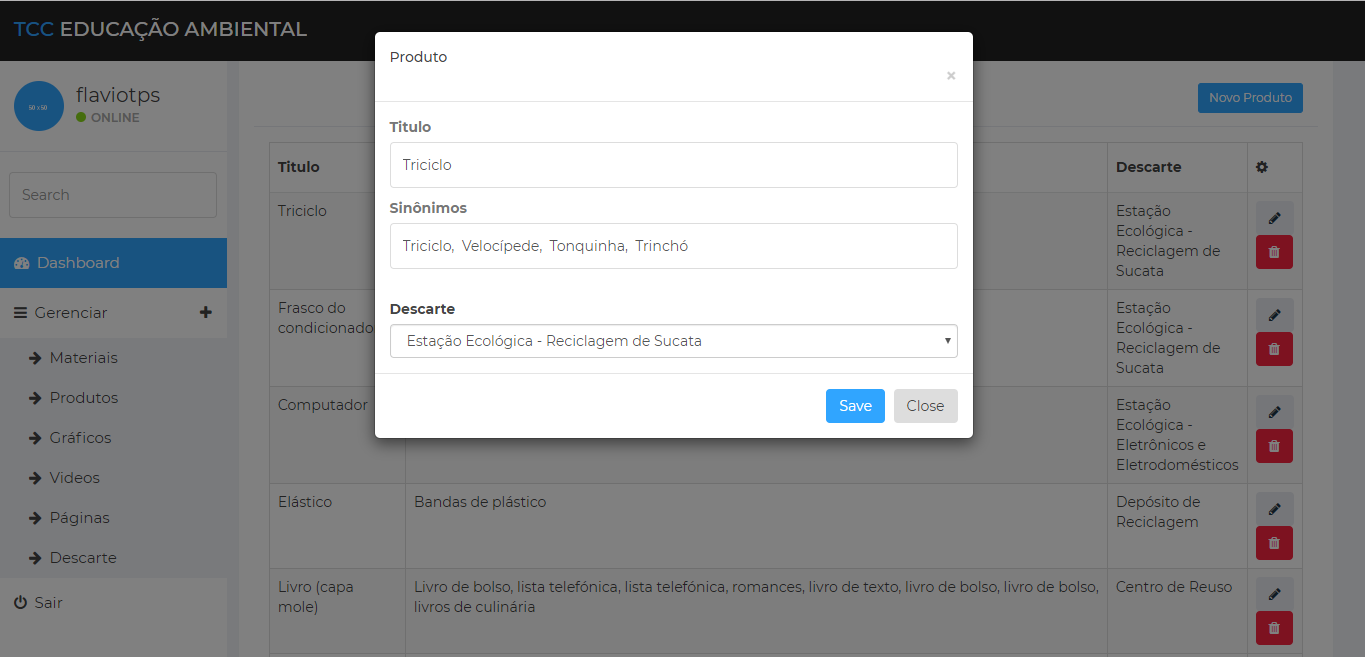
\includegraphics[scale=0.40]{media/tela_produto_site_2.png}
   \legend{Fonte: Autor}
     \label{fig:tela_produto_site_2}
\end{figure}

\newpage
\subsubsection{Tela de estatísticas} \label{tela_stats}
A \autoref{fig:tela_graficos_site_1} e \autoref{fig:tela_graficos_site_2} apresentam a área de estatísticas, que permitem adicionar gráficos do tipo \textit{PieChart} ou \textit{BarChart}. Os dados exibidos devem seguir uma sintaxe para que sejam exibidos corretamente.

\begin{figure}[h]
\centering
   \caption{Gráfico - Todos}
   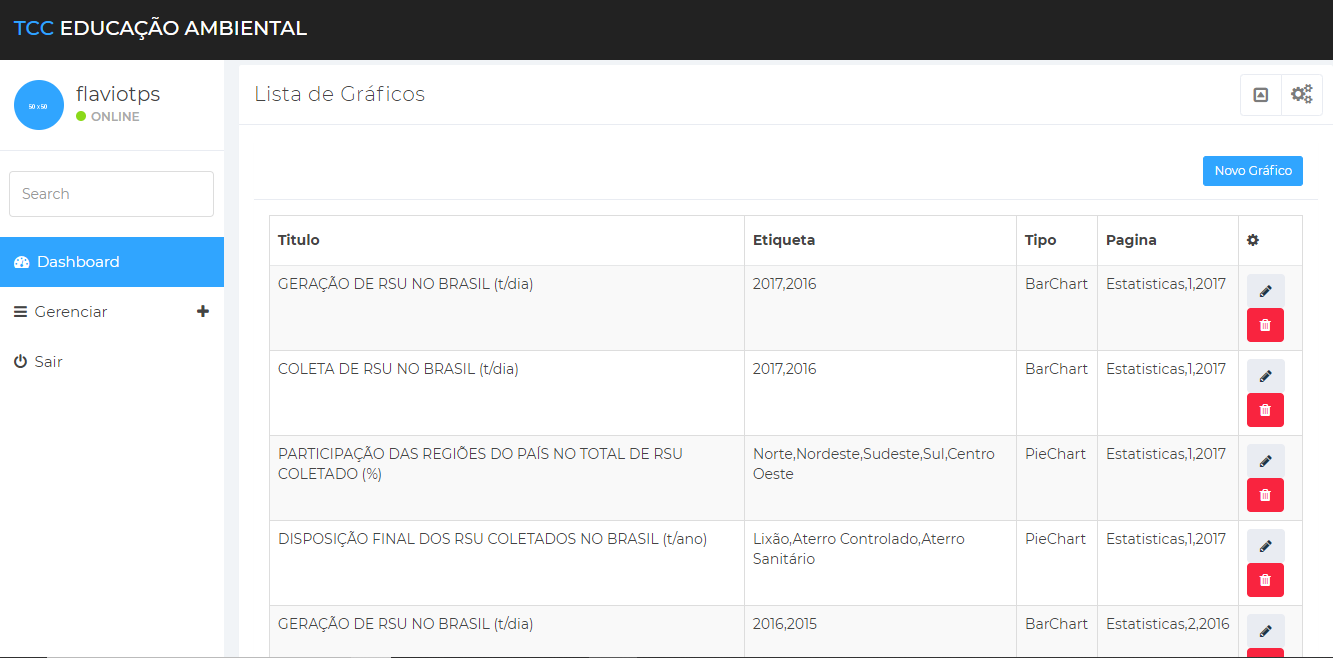
\includegraphics[scale=0.45]{media/tela_graficos_site_1.png}
   \legend{Fonte: Autor}
     \label{fig:tela_graficos_site_1}
\end{figure}

\begin{figure}[h]
\centering
   \caption{Gráfico - Edição}
   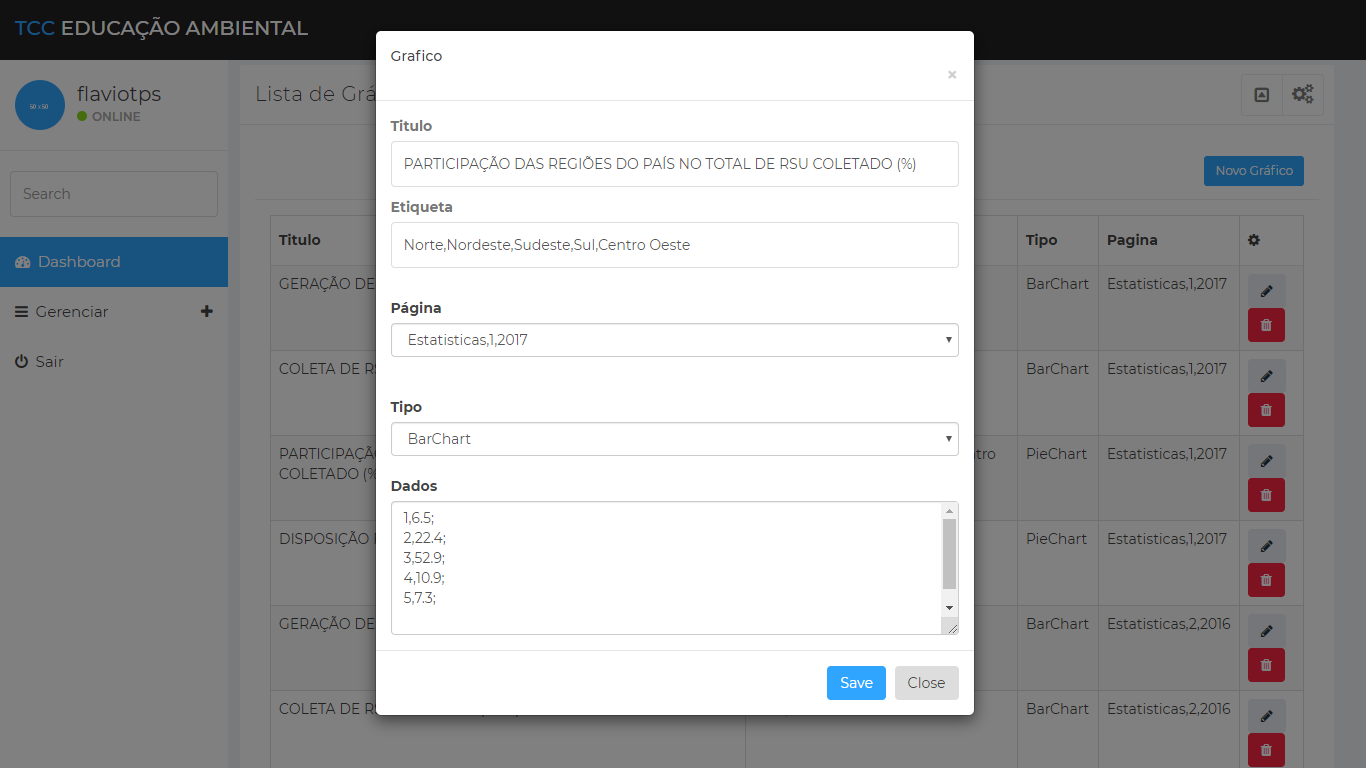
\includegraphics[scale=0.40]{media/tela_graficos_site_2.png}
   \legend{Fonte: Autor}
     \label{fig:tela_graficos_site_2}
\end{figure}

\newpage
\subsubsection{Tela de vídeos} \label{tela_video}
A \autoref{fig:tela_video_site_1} e \autoref{fig:tela_video_site_2} apresentam área de vídeos. Nesta área é possível adicionar vídeos do \textit{youtube} relacionados ao tema através de um \textit{link}. O vídeo fica disponível na seção do vídeos do aplicativo. 

\begin{figure}[h]
\centering
   \caption{Vídeo - Todos}
   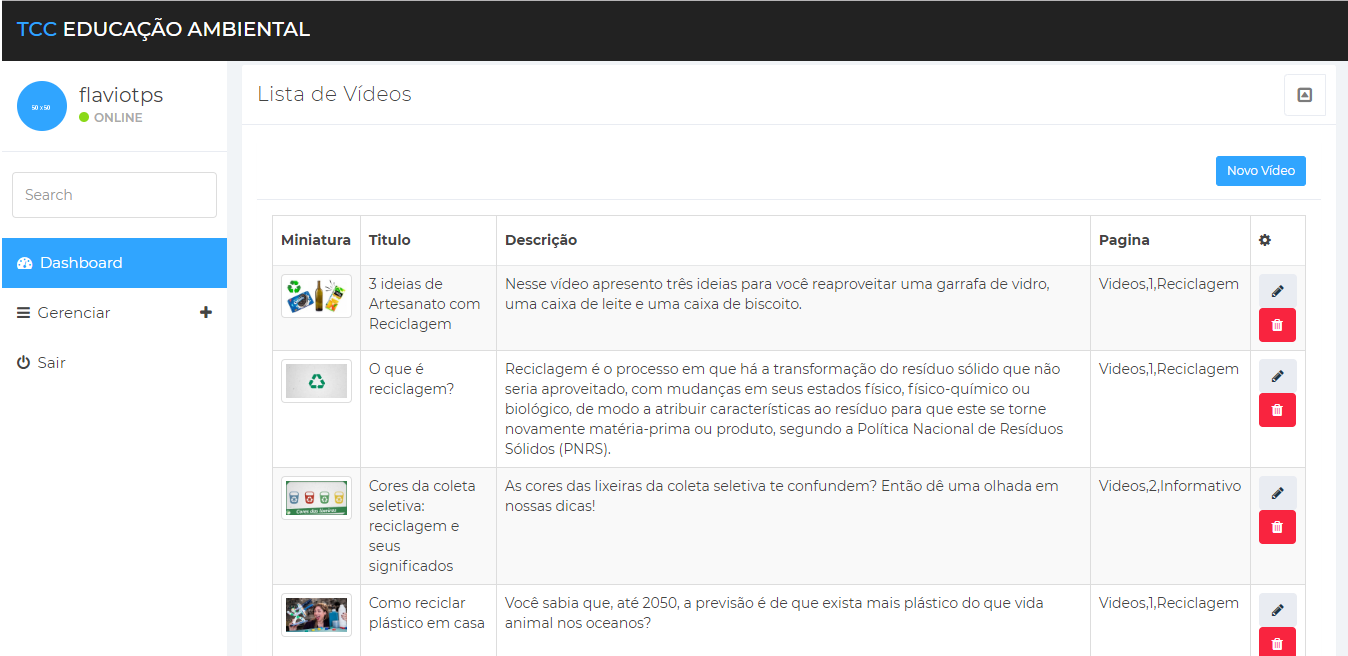
\includegraphics[scale=0.40]{media/tela_video_site_1.png}
   \legend{Fonte: Autor}
     \label{fig:tela_video_site_1}
\end{figure}

\begin{figure}[h]
\centering
   \caption{Vídeo - Edição}
   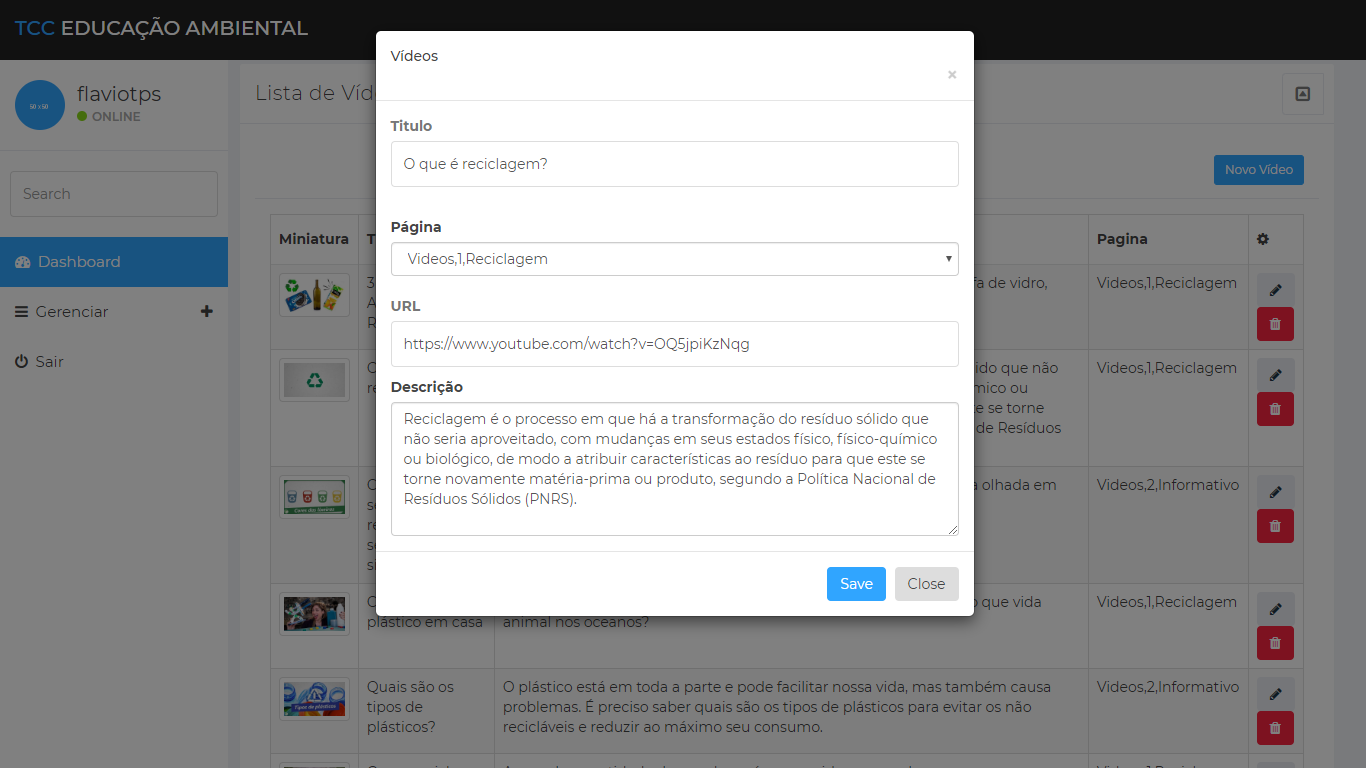
\includegraphics[scale=0.40]{media/tela_video_site_2.png}
   \legend{Fonte: Autor}
     \label{fig:tela_video_site_2}
\end{figure}

\newpage
\subsubsection{Tela de páginas} \label{tela_paginas}
 A \autoref{fig:tela_pagina_site_1} e \autoref{fig:tela_pagina_site_2} apresentam a área onde é possível criar páginas. As áreas de vídeos e gráficos fazem uso desse recurso para organização do conteúdo.

\begin{figure}[h]
\centering
   \caption{Página - Todas}
   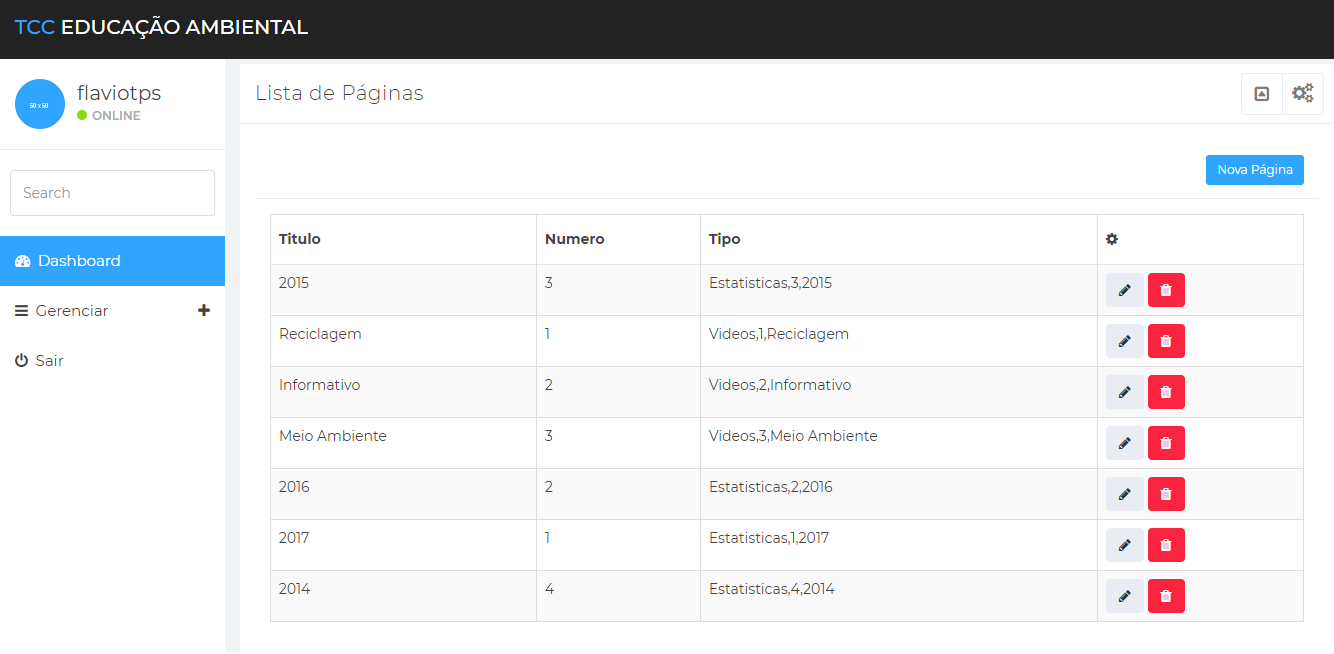
\includegraphics[scale=0.40]{media/tela_pagina_site_1.png}
   \legend{Fonte: Autor}
     \label{fig:tela_pagina_site_1}
\end{figure}

\begin{figure}[h]
\centering
   \caption{Página - Edição}
   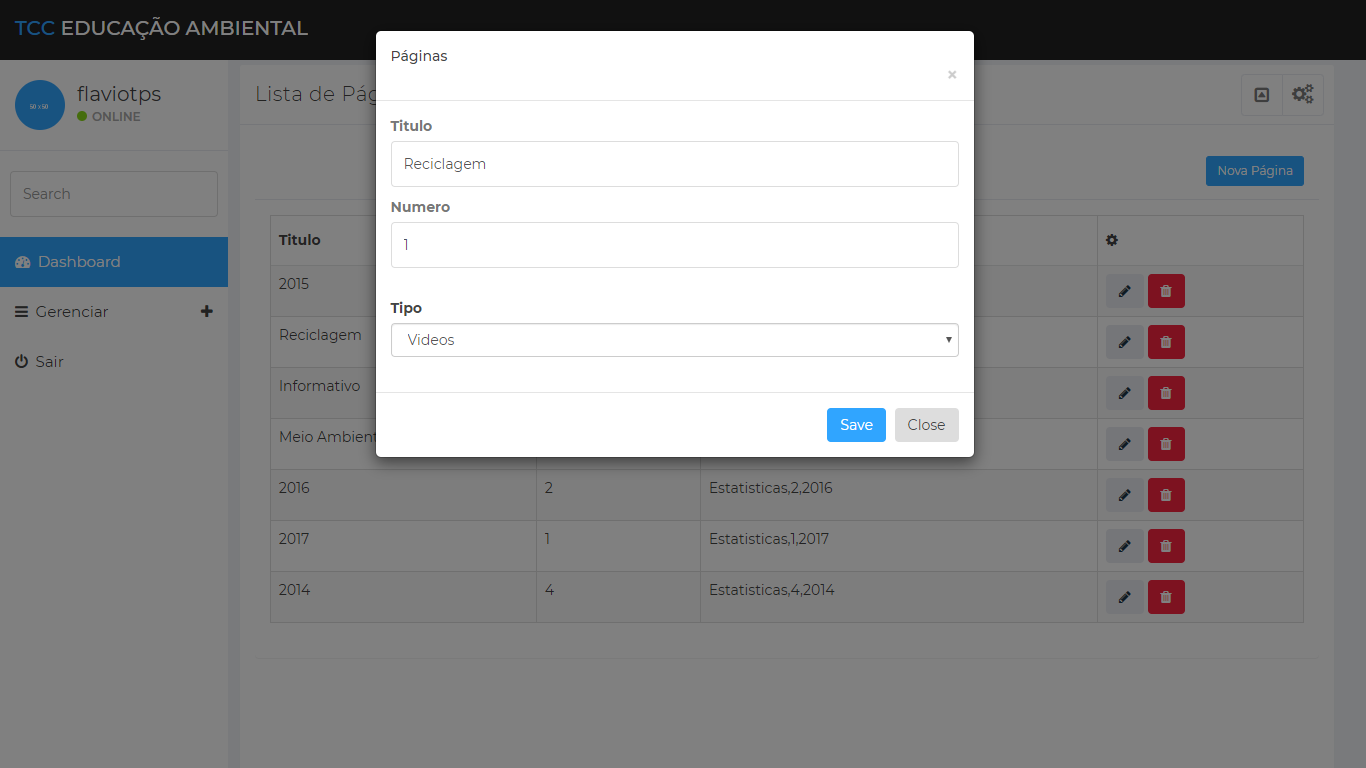
\includegraphics[scale=0.40]{media/tela_pagina_site_2.png}
   \legend{Fonte: Autor}
     \label{fig:tela_pagina_site_2}
\end{figure}
\newpage
\subsubsection{Tela de descartes} \label{tela_descarte}
A \autoref{fig:tela_descarte_site_1} e \autoref{fig:tela_descarte_site_2} apresentam a área onde é possível criar formas de descarte para materiais. A área de produtos faz uso desse recurso.

\begin{figure}[h]
\centering
   \caption{Descarte - Todos}
   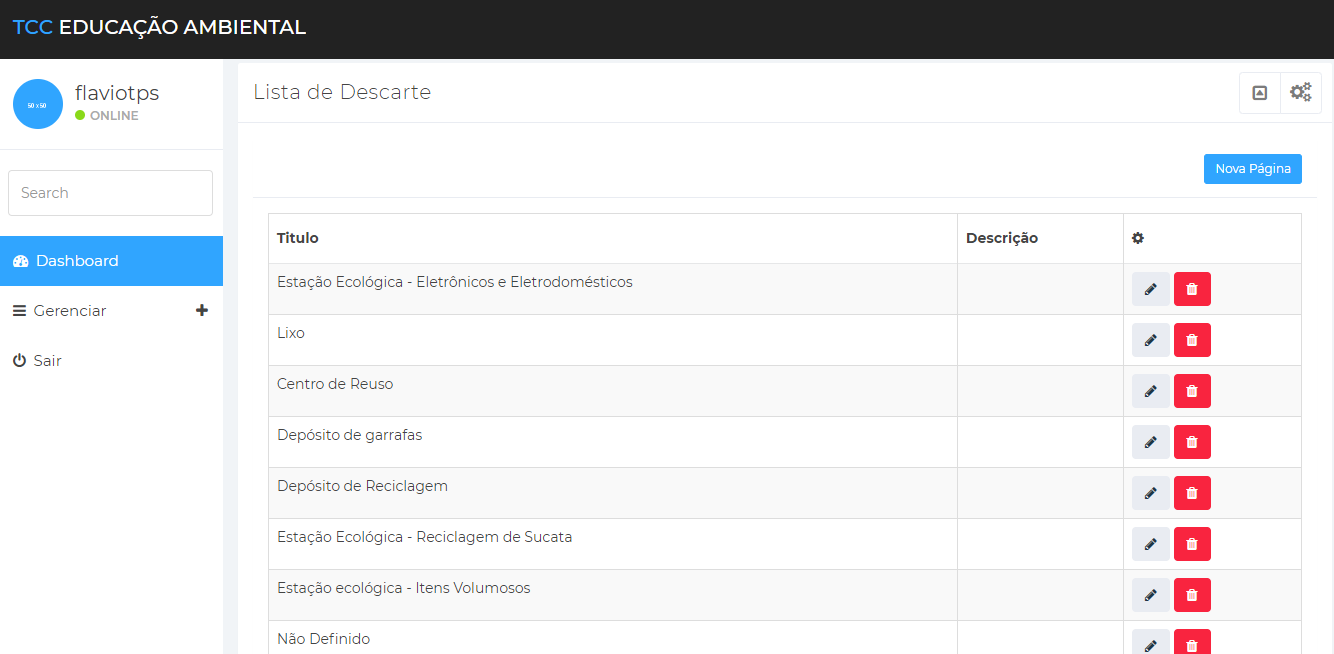
\includegraphics[scale=0.40]{media/tela_descarte_site_1.png}
   \legend{Fonte: Autor}
     \label{fig:tela_descarte_site_1}
\end{figure}

\begin{figure}[h]
\centering
   \caption{Descarte - Edição}
   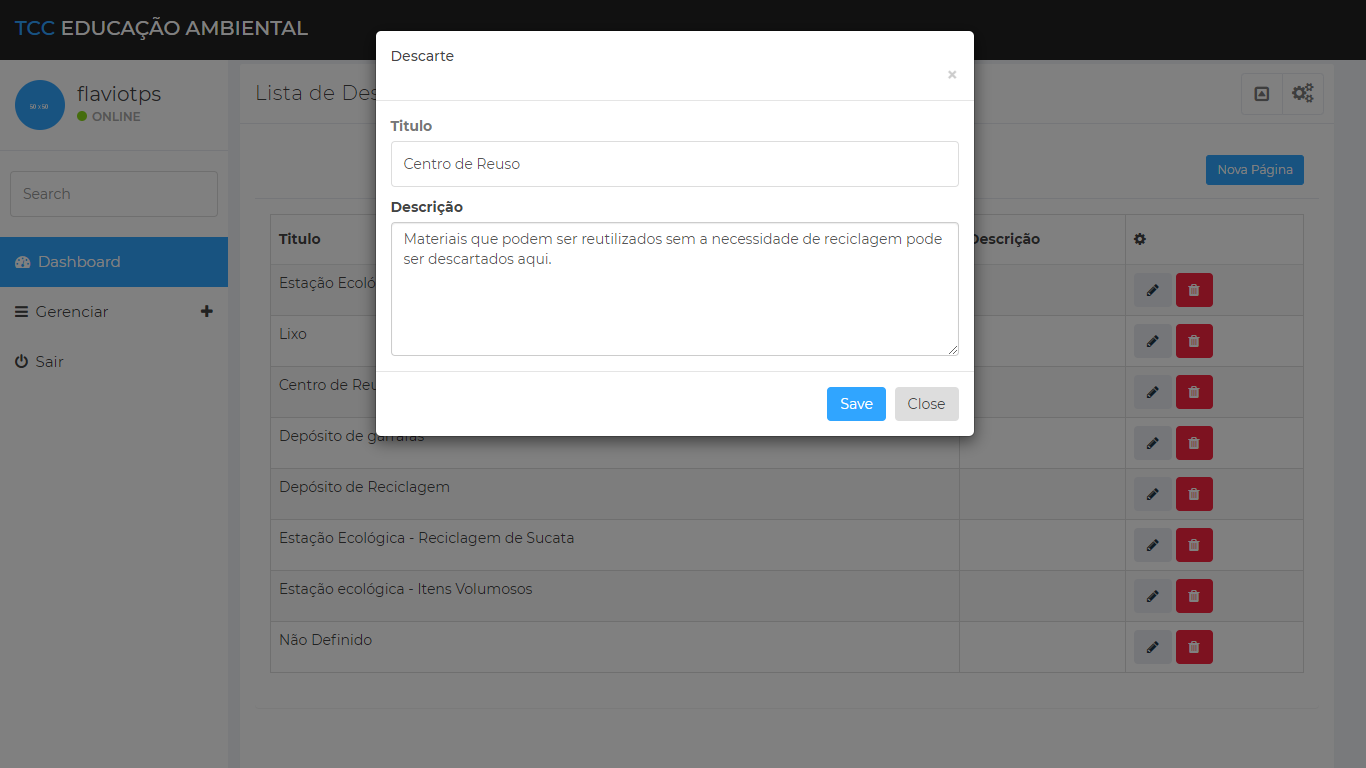
\includegraphics[scale=0.40]{media/tela_descarte_site_2.png}
   \legend{Fonte: Autor}
     \label{fig:tela_descarte_site_2}
\end{figure}
\newpage
\subsection{Aplicativo}
Durante o processo de desenvolvimento foi utilizado arquivos \textit{XML} e \textit{Java}. Os arquivos \textit{Java} são responsáveis por capturar os eventos do sistema e modelar as entidades, enquanto os \textit{XML} ficam responsáveis por desenhar a interface gráfica do aplicativo. O código fonte está disponível em \url{https://github.com/flaviotps/Reciclando_App}.

\subsubsection{Tela de carregamento} \label{splash_activity}
A tela de carregamento, representada pela \autoref{fig:tela_splash_1_app} e \autoref{fig:tela_splash_2_app}, foi desenvolvida para carregar os dados que serão utilizados no aplicativo de forma paralela. Nesta etapa há uma verificação de conectividade. Caso haja conexão com a internet o método \textit{getData} procura por atualizações. Caso não haja conexão, os últimos dados carregados serão utilizados.
As animações de carregamento foram desenvolvidas utilizando a biblioteca Lottie.



    \begin{figure}[htb]    
 \centering
  \begin{minipage}{0.5\textwidth}
    \centering
    \caption{Carregando}
    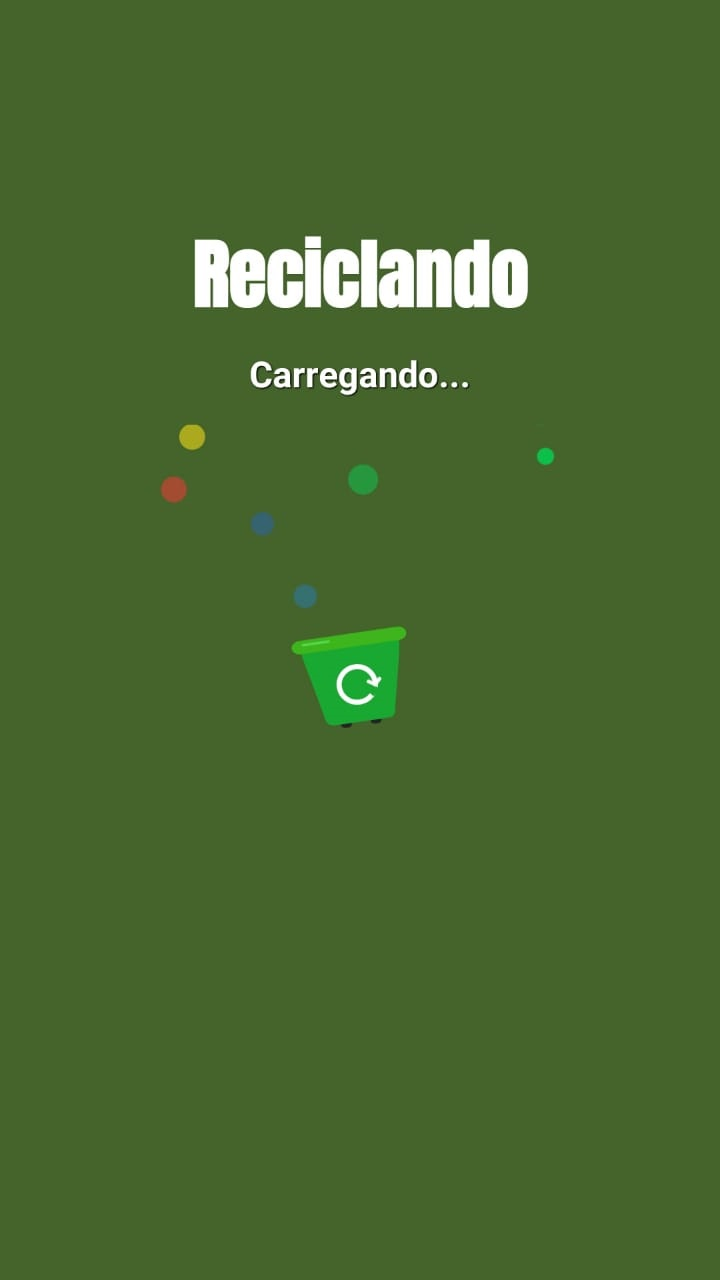
\includegraphics[scale=0.35]{media/tela_splash_1.jpg}
    \legend{Fonte: Autor}
     \label{fig:tela_splash_1_app}
  \end{minipage}
  \hfill
  \begin{minipage}{0.45\textwidth}
    \centering
    \caption{Carregado}
    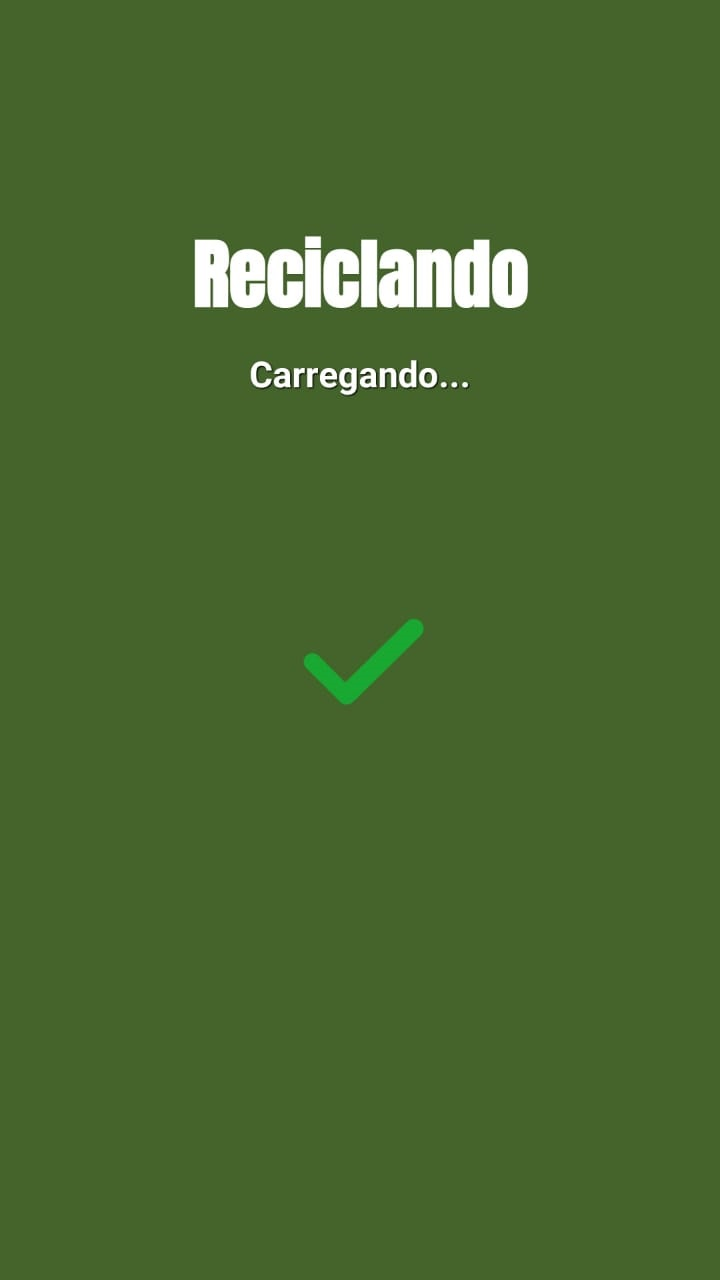
\includegraphics[scale=0.35]{media/tela_splash_2.jpg}
    \legend{Fonte: Autor}
     \label{fig:tela_splash_2_app}
  \end{minipage}
\end{figure}

\newpage
\subsubsection{Tela Principal} \label{main_activity}
Após o carregamento dos dados na \nameref{splash_activity} o usuário é redirecionado para a \nameref{fig:activity_main_app}. Essa \nameref{activity} é responsável por criar vários \nameref{fragment} que levam o usuário para diferentes partes do aplicativo através de um menu (\textit{BottomNavigationView}). Para melhorar a experiência do usuário foi utilizado também um \nameref{ViewPager} que é configurado no método \textit{setupViewPager}, o que possibilita uma troca de conteúdo rápido de acordo com as ações do usuário que são controladas pelo método \textit{onNavigationItemSelected} ou pelo \textit{onPageSelected}. Por padrão a Tela Principal possui somente o \textit{BottomNavigationView} e \nameref{ViewPager}, o \nameref{fragment} padrão é adicionado em tempo de execução. Neste caso, usamos o \nameref{main_fragment}.


\begin{figure}[h]
\centering
   \caption{Tela Principal}
   
\includegraphics[scale=1.0]{media/activity_main.png}
   \legend{Fonte: Autor}
     \label{fig:activity_main_app}
\end{figure}

\newpage
\subsubsection{Tela Menu Principal} \label{main_fragment}
A \nameref{fig:fragment_main_app} é responsável por criar o menu principal do aplicativo e controlar as ações do usuário através da interface \textit{OnClickListener}, que responde aos cliques do usuário na interface gráfica. Esse \nameref{fragment} pode realizar alterações no \nameref{ViewPager} da \nameref{main_activity} e abrir novas telas.

\begin{figure}[h]
\centering
   \caption{Tela Menu Principal}
   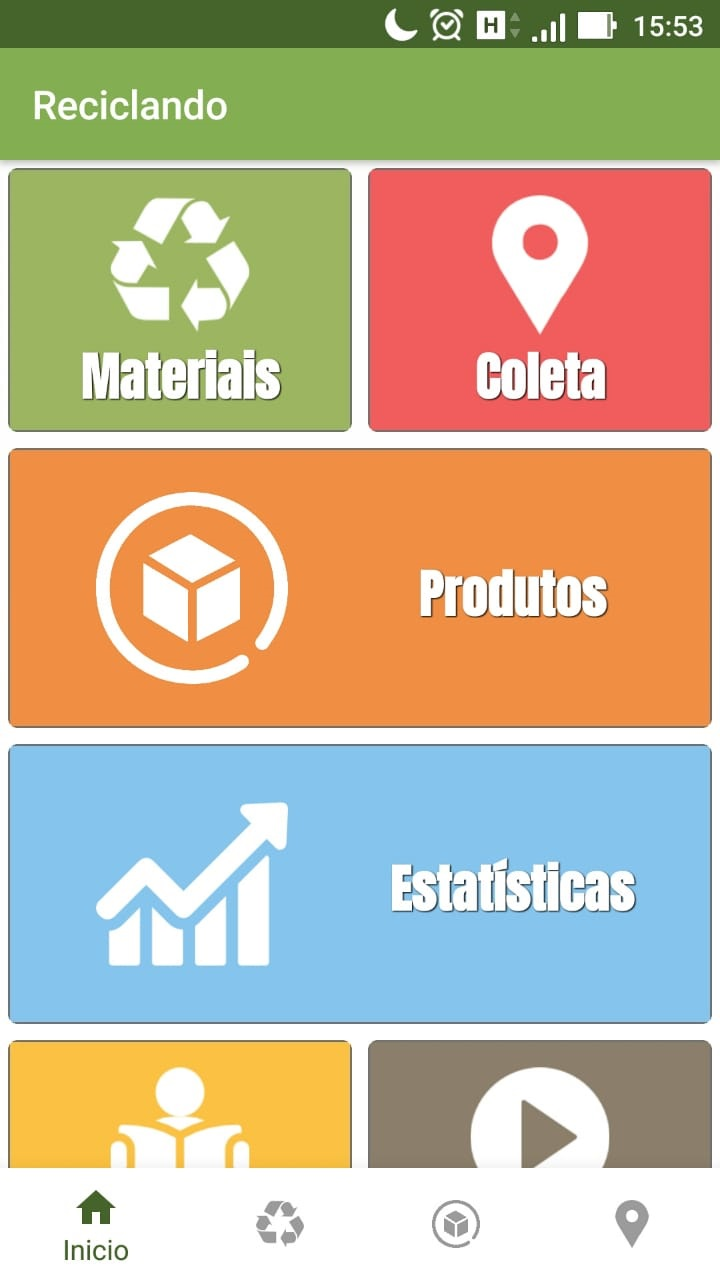
\includegraphics[scale=0.4]{media/fragment_main.jpg}
   \legend{Fonte: Autor}
     \label{fig:fragment_main_app}
\end{figure}

\newpage
\subsubsection{Tela Menu de Materiais} \label{FragmentMaterialMenu}
Ao selecionar a opção de materiais, o \nameref{main_activity} troca o \nameref{fragment} e exibe o \nameref{fig:tela_menu_material_1}, que é o \nameref{fragment} responsável por exibir o menu de materiais específicos e controlar as ações do usuário neste menu. Ao clicar em um dos menus disponíveis o método \textit{onClick} da \textit{interface} \textit{OnClickListener} é acionado e a informação do material é passada para próxima tela através do \nameref{Intent}.
\
    \begin{figure}[htb]    
 \centering
  \begin{minipage}{0.45\textwidth}
    \centering
    \caption{Tela Menu de Materiais}
    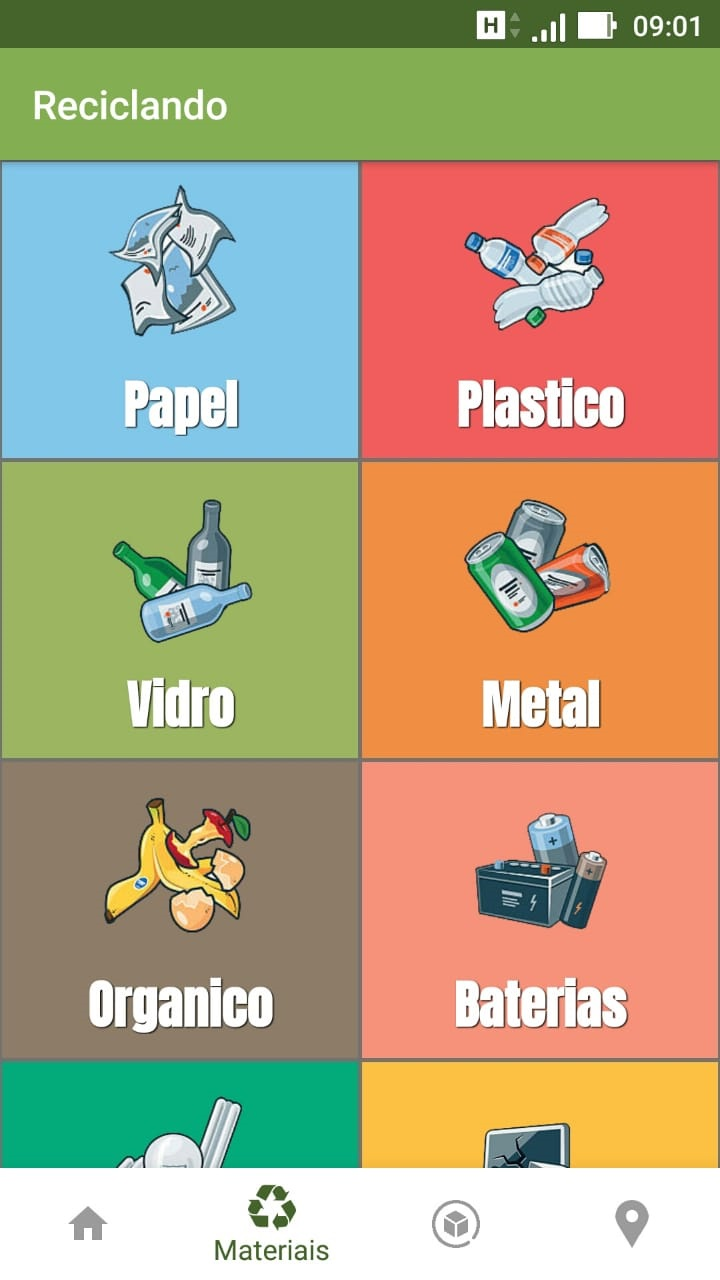
\includegraphics[scale=0.45]{media/tela_menu_material_1.jpg}
    \legend{Fonte: Autor}
     \label{fig:tela_menu_material_1}
  \end{minipage}
  \hfill
\end{figure}

\newpage
\subsubsection{Tela de Materiais} \label{ActivityMaterial}
A tela de materiais, ilustrada pela \autoref{fig:tela_material_act_1} e \autoref{fig:tela_material_act_2}, é utilizada para exibir um \nameref{RecyclerView} de materiais recicláveis e um campo de busca para filtrar os resultados carregados.

Essa \nameref{activity} é criada a partir de um \nameref{Intent} que recebe como parâmetro o tipo do material. Com esse parâmetro todos os materiais são filtrados e o \nameref{RecyclerView} é construído.

    \begin{figure}[htb]    
 \centering
  \begin{minipage}{0.45\textwidth}
    \centering
    \caption{Tela de Materiais -  Plásticos}
    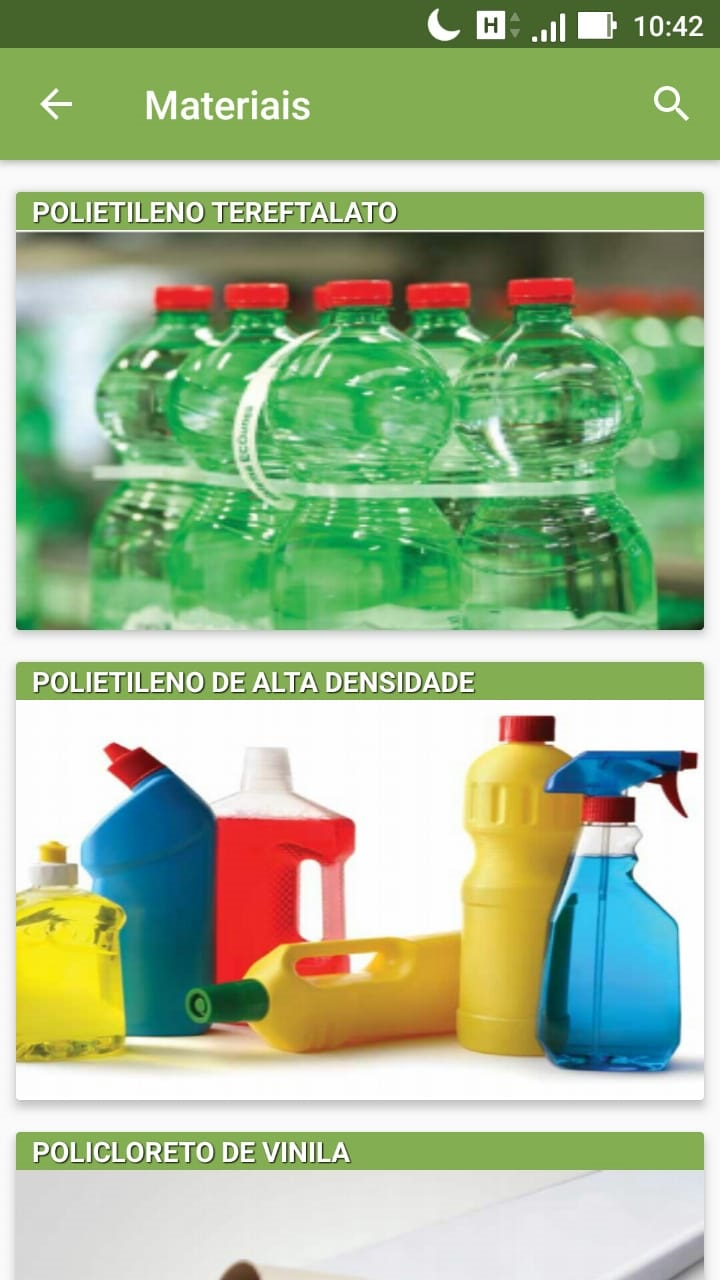
\includegraphics[scale=0.35]{media/tela_material_act_1.jpg}
    \legend{Fonte: Autor}
     \label{fig:tela_material_act_1}
  \end{minipage}
  \hfill
  \begin{minipage}{0.45\textwidth}
    \centering
    \caption{Tela de Materiais -  Plásticos}
    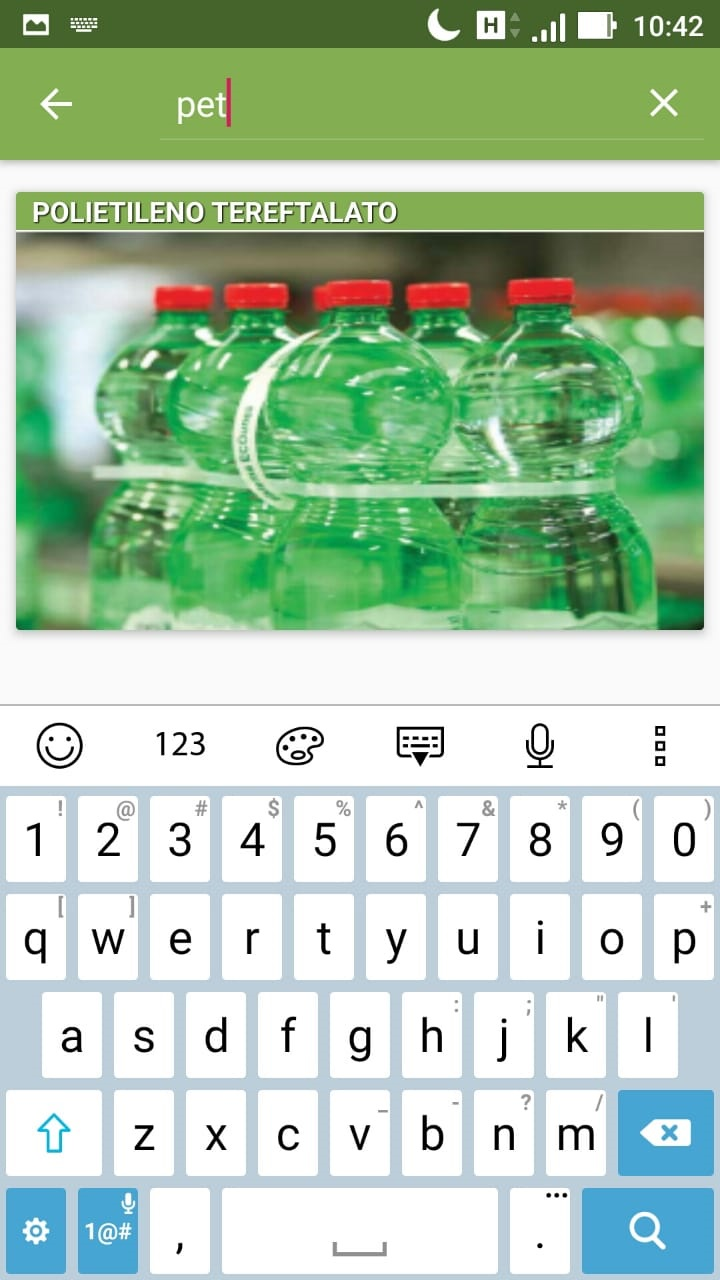
\includegraphics[scale=0.35]{media/tela_material_act_2.jpg}
    \legend{Fonte: Autor}
     \label{fig:tela_material_act_2}
  \end{minipage}
\end{figure}

\newpage
\subsubsection{Tela Detalhes de Materiais} \label{ActivityMaterialDetails}
Quando um item da \nameref{ActivityMaterial} é selecionado a tela de detalhes de materiais, representada pela \autoref{fig:tela_material__details_act_1}, é aberta através de um \nameref{Intent} que leva os dados do material a ser exibido. Essa \nameref{activity} exibe o conteúdo dos dados do material em HTML através de um \nameref{WebView}.

    \begin{figure}[htb]    
 \centering
  \begin{minipage}{0.45\textwidth}
    \centering
    \caption{Tela Detalhes de Materiais}
    \includegraphics[scale=0.45]{media/tela_material__details_act_1.jpg}
    \legend{Fonte: Autor}
     \label{fig:tela_material__details_act_1}
  \end{minipage}
  \hfill
\end{figure}

\newpage
\subsubsection{Tela de Estatísticas}
\label{ActivityStatistics}
A tela de estatísticas, ilustrada na \autoref{fig:tela_stats_1} e \autoref{fig:tela_stats_2}, também faz uso do \nameref{ViewPager} com \nameref{fragment} para alternar o conteúdo exibido. Neste caso utilizamos um \nameref{TabLayout} para alternar entre o conteúdo. O \nameref{TabLayout} é construído a partir de informações carregadas no \nameref{Sistema Administrativo}, o que possibilita a criação de categorias de forma dinâmica. Quando uma categoria do \nameref{TabLayout} é selecionada a Tela de Estatísticas cria um \nameref{fragment} com o argumento identificador da página no seu \nameref{Bundle} e exibe o conteúdo através de um \nameref{RecyclerView}.
  
    \begin{figure}[htb]    
 \centering
  \begin{minipage}{0.45\textwidth}
    \centering
    \caption{Tela de Estatísticas}
    \includegraphics[scale=0.35]{media/tela_stats_1.jpg}
    \legend{Fonte: Autor}
     \label{fig:tela_stats_1}
  \end{minipage}
  \hfill
  \begin{minipage}{0.45\textwidth}
    \centering
    \caption{Tela de Estatísticas}
    \includegraphics[scale=0.35]{media/tela_stats_2.jpg}
    \legend{Fonte: Autor}
     \label{fig:tela_stats_2}
  \end{minipage}
\end{figure}

\newpage
\subsubsection{Tela de Vídeos}
A tela de vídeos, ilustrada na \autoref{fig:tela_videos_1} e \autoref{fig:tela_videos_2}, utiliza um \nameref{ViewPager}, \nameref{TabLayout} e \nameref{fragment} para disponibilizar uma lista de vídeos usando um \nameref{RecyclerView}. As informações são carregadas diretamente do \textit{Youtube}. Os vídeos podem ser reproduzidos ao clicar em suas imagens ou descrição.

    \begin{figure}[htb]    
 \centering
  \begin{minipage}{0.45\textwidth}
    \centering
    \caption{Tela de Vídeos}
    \includegraphics[scale=0.35]{media/tela_videos_1.jpg}
    \legend{Fonte: Autor}
     \label{fig:tela_videos_1}
  \end{minipage}
  \hfill
  \begin{minipage}{0.45\textwidth}
    \centering
    \caption{Tela de Vídeos}
    \includegraphics[scale=0.35]{media/tela_videos_2.jpg}
    \legend{Fonte: Autor}
     \label{fig:tela_videos_2}
  \end{minipage}
\end{figure}

\newpage
\subsubsection{Tela de Locais}
A Tela de Locais utiliza um \nameref{MapView} e \nameref{RecyclerView} para disponibilizar uma lista de pontos de interesse e exibi-los no mapa. As localizações são carregadas diretamente da \nameref{API} do Google. A \autoref{fig:tela_location_1} e \autoref{fig:tela_location_2} ilustram essa tela.

    \begin{figure}[htb]    
 \centering
  \begin{minipage}{0.45\textwidth}
    \centering
    \caption{Coleta}
    \includegraphics[scale=0.35]{media/tela_location_1.jpeg}
    \legend{Fonte: Autor}
     \label{fig:tela_location_1}
  \end{minipage}
  \hfill
  \begin{minipage}{0.45\textwidth}
    \centering
    \caption{Coleta}
    \includegraphics[scale=0.35]{media/tela_location_2.jpeg}
    \legend{Fonte: Autor}
     \label{fig:tela_location_2}
  \end{minipage}
\end{figure}
\end{chapter}

\newpage

\subsubsection{Tela de produtos}
A \autoref{fig:produtos_app} ilustra a tela de produtos, onde uma lista de produtos com informações de descarte adequado é exibida. É possível filtrar um produto por nome ou sinônimos.



\begin{figure}[htb]    
 \centering
  \begin{minipage}{0.55\textwidth}
    \centering
    \caption{Tela de Produtos}
    \includegraphics[scale=0.35]{media/produtos_app.jpeg}
    \legend{Fonte: Autor}
     \label{fig:produtos_app}
  \end{minipage}
  \hfill
\end{figure}


% ----------------------------------------------------------
\chapter{Conclusão}
Este trabalho apresentou o desenvolvimento de um aplicativo voltado a educação ambiental utilizando tecnologias como Android, GPS e Firebase. Para atingir o objetivo de desenvolvimento de um aplicativo que demonstra, através de vídeos, gráficos e textos, o impacto que os resíduos descartados de forma incorreta podem causar, foi necessário passar pelas etapas de modelagem do sistema e obter novos conhecimentos. Tanto na linguagem Java quanto no ecossistema de desenvolvimento da Google. Também foi necessário fazer o levantamento de dados para serem inseridos no aplicativo, tais como dados estatísticos, informações sobre os materiais, vídeos e aprender como disponibilizar esses dados para o aplicativo usando o conceito de API e o padrão JSON.

As principais dificuldades encontradas durante o desenvolvimento do projeto foi a integração com as ferramentas da Google, como o Firebase e Google Maps. Devido à quantidade de opções disponíveis nessa infraestrutura, o processo de escolha e entendimento das ferramentas se torna confuso para quem está iniciando o desenvolvimento com tais ferramentas.
A versão final do aplicativo encontra-se disponível na Google Play através do \textit{link} \href{https://play.google.com/store/apps/details?id=com.flaviotps.reciclando}{https://play.google.com/store/apps/details?id=com.flaviotps.reciclando}.

% ----------------------------------------------------------
\section{Trabalhos futuros}
O aplicativo desenvolvido apresenta as funções necessárias para atender o propósito do trabalho. Mas devido à constante evolução do ecossistema da Google, o aplicativo precisará passar pela migração para linguagem Kotlin e novas diretrizes da Google, para que seja compatível com as futuras versões do Android.

Outras funcionalidades também serão implementadas, como a funcionalidade destinada ao entendimento de nomenclaturas e padrões utilizados no descarte e identificação de resíduos. Como por exemplo, as cores características dos contêineres de coleta seletiva de lixo e a classificação numérica dos tipos de plásticos. 
Essa funcionalidade será inserida no menu "Aprenda", localizado na \nameref{main_fragment} do aplicativo.

% ----------------------------------------------------------
% ELEMENTOS PÓS-TEXTUAIS
% ----------------------------------------------------------
\postextual
% ----------------------------------------------------------

% ----------------------------------------------------------
% Referências bibliográficas
% ----------------------------------------------------------

\bibliographystyle{halpha-abbrv.bst}
\bibliography{bibliography.bib}




% ----------------------------------------------------------
% Glossário
% ----------------------------------------------------------
%
% Consulte o manual da classe abntex2 para orientações sobre o glossário.
%
%\glossary

% ----------------------------------------------------------
% Apêndices
% ----------------------------------------------------------

%\begin{apendicesenv}
%% Imprime uma página indicando o início dos apêndices
%\partapendices
%\end{apendicesenv}



%---------------------------------------------------------------------
% INDICE REMISSIVO
%---------------------------------------------------------------------
\phantompart
\printindex
%---------------------------------------------------------------------

\end{document}
